\documentclass[14pt]{beamer}
\usepackage{./Estilos/BeamerUVM}
\usepackage{./Estilos/ColoresLatex}
\usetheme{Madrid}
\usecolortheme{default}
%\useoutertheme{default}
\setbeamercovered{invisible}
% or whatever (possibly just delete it)
\setbeamertemplate{section in toc}[sections numbered]
\setbeamertemplate{subsection in toc}[subsections numbered]
\setbeamertemplate{subsection in toc}{\leavevmode\leftskip=3.2em\rlap{\hskip-2em\inserttocsectionnumber.\inserttocsubsectionnumber}\inserttocsubsection\par}
% \setbeamercolor{section in toc}{fg=blue}
% \setbeamercolor{subsection in toc}{fg=blue}
% \setbeamercolor{frametitle}{fg=blue}
\setbeamertemplate{caption}[numbered]

\setbeamertemplate{footline}
\beamertemplatenavigationsymbolsempty
\setbeamertemplate{headline}{}


\makeatletter
% \setbeamercolor{section in foot}{bg=gray!30, fg=black!90!orange}
% \setbeamercolor{subsection in foot}{bg=blue!30}
% \setbeamercolor{date in foot}{bg=black}
\setbeamertemplate{footline}
{
  \leavevmode%
  \hbox{%
  \begin{beamercolorbox}[wd=.333333\paperwidth,ht=2.25ex,dp=1ex,center]{section in foot}%
    \usebeamerfont{section in foot} {\insertsection}
  \end{beamercolorbox}%
  \begin{beamercolorbox}[wd=.333333\paperwidth,ht=2.25ex,dp=1ex,center]{subsection in foot}%
    \usebeamerfont{subsection in foot}  \insertsubsection
  \end{beamercolorbox}%
  \begin{beamercolorbox}[wd=.333333\paperwidth,ht=2.25ex,dp=1ex,right]{date in head/foot}%
    \usebeamerfont{date in head/foot} \insertshortdate{} \hspace*{2em}
    \insertframenumber{} / \inserttotalframenumber \hspace*{2ex} 
  \end{beamercolorbox}}%
  \vskip0pt%
}
\makeatother

\makeatletter
\patchcmd{\beamer@sectionintoc}{\vskip1.5em}{\vskip0.8em}{}{}
\makeatother

% \usefonttheme{serif}

\title{\Large{Los polígonos} \\ \normalsize{Matemáticas II}}

\date{14 de abril de 2023}

\begin{document}
\maketitle

\section*{Contenido}
\frame{\frametitle{Contenido} \tableofcontents[currentsection, hideallsubsections]}

\section{Bloque 2}
\frame[allowframebreaks]{\frametitle{Contenido} \tableofcontents[currentsection, hideothersubsections]}
\subsection{Aprendizajes Esperados}

\begin{frame}
\frametitle{Aprendizajes esperados}
Al concluir el Bloque 2, el alumno:
\setbeamercolor{item projected}{bg=lava,fg=white}
\setbeamertemplate{enumerate items}{%
\usebeamercolor[bg]{item projected}%
\raisebox{1.5pt}{\colorbox{bg}{\color{fg}\footnotesize\insertenumlabel}}%
}
\begin{enumerate}[<+->]
\item Desarrolla estrategias colaborativamente, para la solución de problemas utiliznado los elementos y propiedades de \textocolor{ao}{polígonos} y \textocolor{carmine}{poliedros} que le permitan cuantificar el espacio en situaciones de su contexto.
\seti
\end{enumerate}
\end{frame}
\begin{frame}
\frametitle{Aprendizajes esperados}
\setbeamercolor{item projected}{bg=lava,fg=white}
\setbeamertemplate{enumerate items}{%
\usebeamercolor[bg]{item projected}%
\raisebox{1.5pt}{\colorbox{bg}{\color{fg}\footnotesize\insertenumlabel}}%
}
\begin{enumerate}[<+->]
\conti
\item Examina las figuras geométricas en diferentes expresiones artísticas.
\end{enumerate}
\end{frame}

\subsection{Habilidades}

\begin{frame}
\frametitle{Habilidades}
\setbeamercolor{item projected}{bg=ao,fg=white}
\setbeamertemplate{enumerate items}{%
\usebeamercolor[bg]{item projected}%
\raisebox{1.5pt}{\colorbox{bg}{\color{fg}\footnotesize\insertenumlabel}}%
}
\begin{enumerate}[<+->]
\item Clasifica polígonos y representa los elementos que los conforman.
\item Argumenta cuáles elementos de los polígonos deberían de utilizarse para solucionar problemas de su entorno.
\seti
\end{enumerate}
\end{frame}
\begin{frame}
\frametitle{Habilidades}
\setbeamercolor{item projected}{bg=ao,fg=white}
\setbeamertemplate{enumerate items}{%
\usebeamercolor[bg]{item projected}%
\raisebox{1.5pt}{\colorbox{bg}{\color{fg}\footnotesize\insertenumlabel}}%
}
\begin{enumerate}[<+->]
\conti
\item Identifica perímetros, áreas y volúmenes de cuerpos geométricos planos y en el espacio.
\item Describe figuras geométricas en las diferentes representaciones artísticas.
\end{enumerate}
\end{frame}

\subsection{Conocimientos}

\begin{frame}
\frametitle{Temas a revisar}
Polígonos.
\pause
\setbeamercolor{item projected}{bg=bananayellow,fg=black}
\setbeamertemplate{enumerate items}{%
\usebeamercolor[bg]{item projected}%
\raisebox{1.5pt}{\colorbox{bg}{\color{fg}\footnotesize\insertenumlabel}}%
}
\begin{enumerate}[<+->]
\item Elementos y clasificación.
\item Ángulo central.
\item Ángulo interior.
\item Ángulo exterior.
\item Suma de ángulos interiores, exteriores.
\item Diagonales.
\item Perímetros y áreas.
\end{enumerate}
\end{frame}
\begin{frame}
\frametitle{Temas a revisar}
Poliedros.
\pause
\setbeamercolor{item projected}{bg=blue-violet,fg=white}
\setbeamertemplate{enumerate items}{%
\usebeamercolor[bg]{item projected}%
\raisebox{1.5pt}{\colorbox{bg}{\color{fg}\footnotesize\insertenumlabel}}%
}
\begin{enumerate}[<+->]
\item Elementos y clasificación.
\item Volúmenes.
\end{enumerate}
\end{frame}

\section{Polígonos en la vida diaria}
\frame{\frametitle{Contenido} \tableofcontents[currentsection, hideothersubsections]}
\subsection{Naturaleza, Vida Diaria, Arte}

\begin{frame}
\frametitle{En la naturaleza}
\begin{figure}
    \centering
    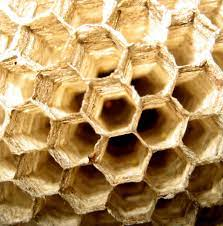
\includegraphics[scale=0.8]{Imagenes/Panel_Abejas_Hexagonal.jpg}
\end{figure}
\end{frame}
\begin{frame}
\frametitle{En la naturaleza}
\begin{figure}
    \centering
    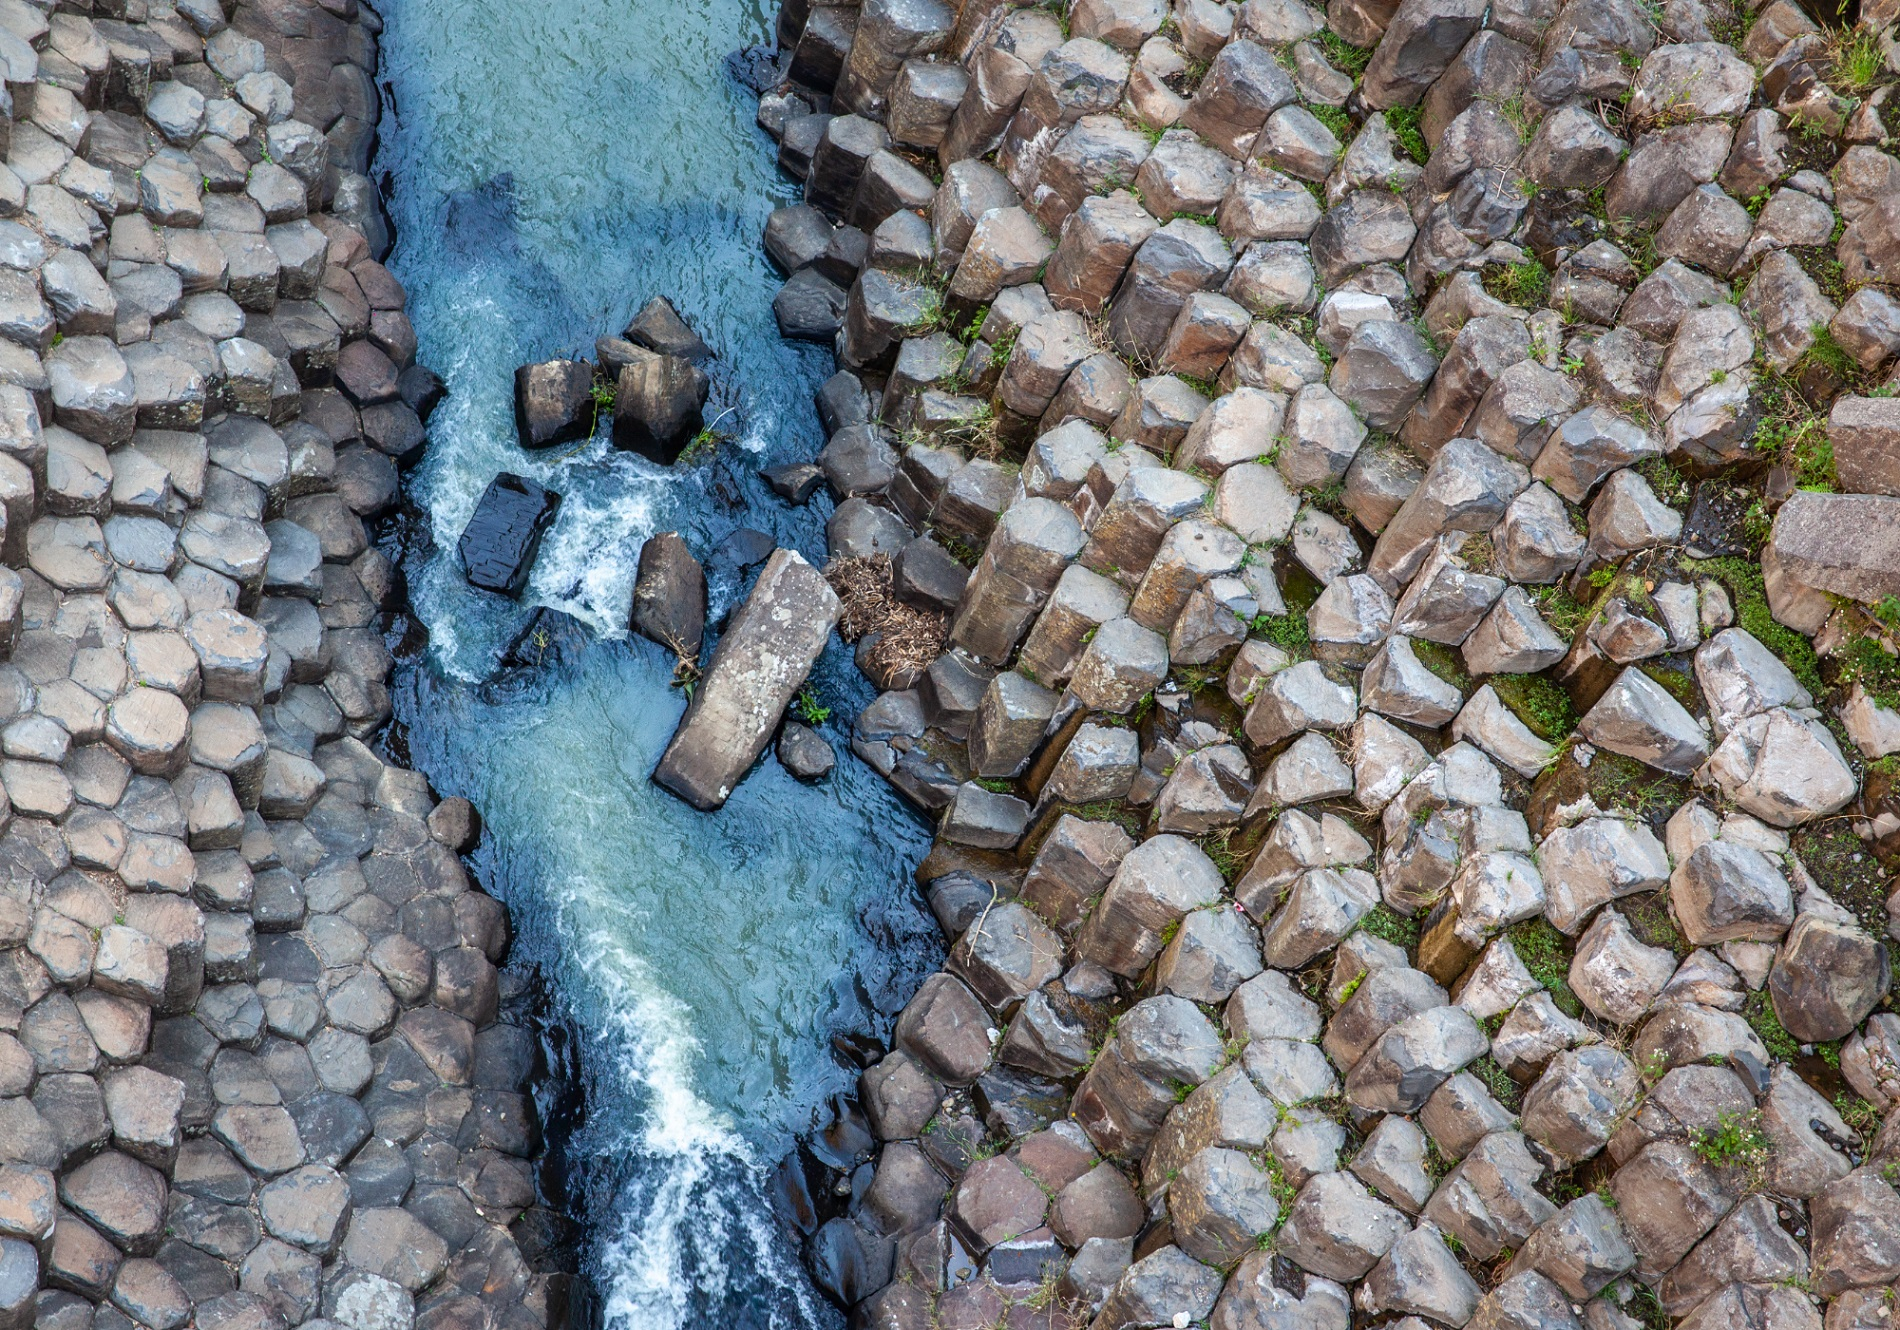
\includegraphics[scale=0.25]{Imagenes/Prismas_Basalticos.jpg}
\end{figure}
\end{frame}

\begin{frame}
\frametitle{En la vida diaria}
\begin{figure}
    \centering
    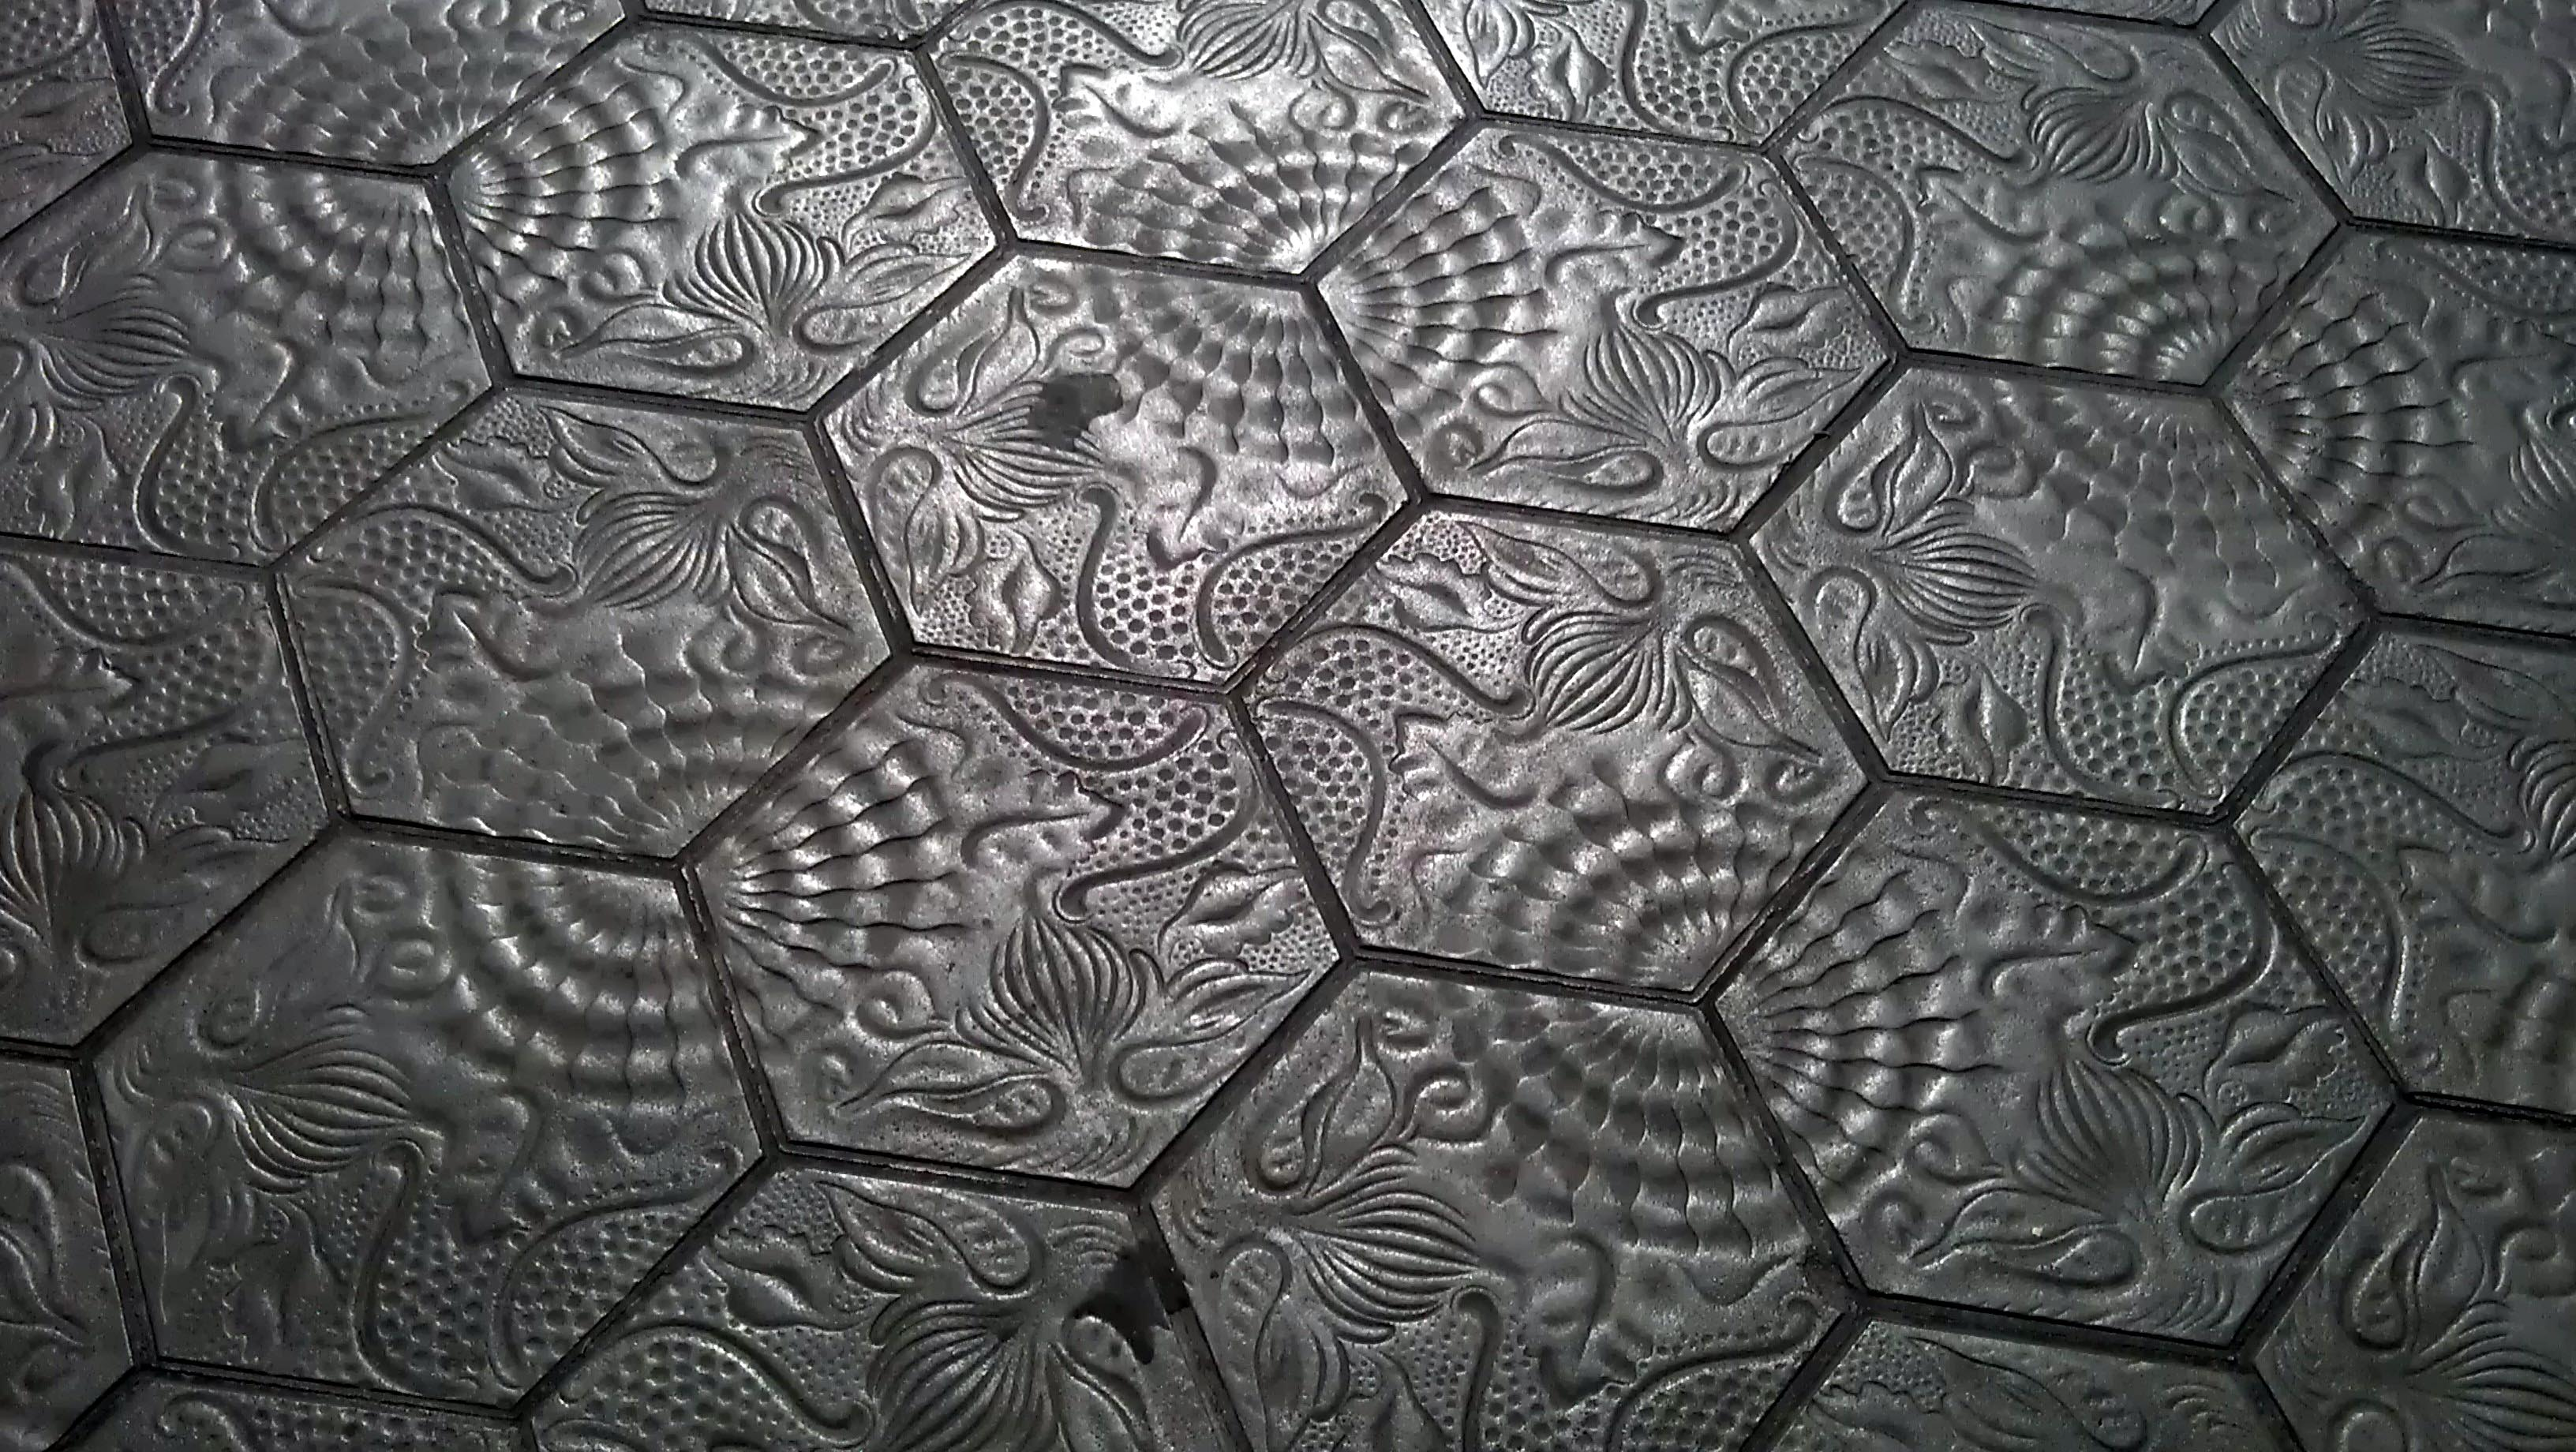
\includegraphics[scale=0.1]{Imagenes/Piso_hexagonal.jpg}
\end{figure}
\end{frame}
\begin{frame}
\frametitle{En la vida diaria}
\begin{figure}
    \centering
    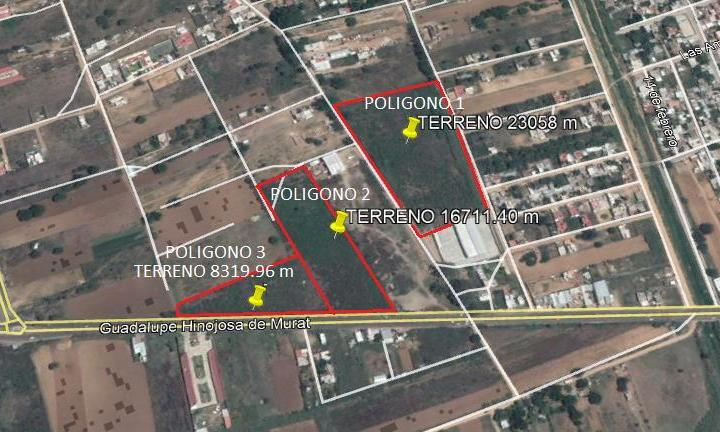
\includegraphics[scale=0.5]{Imagenes/Terrenos_Poligonales.jpg}
\end{figure}
\end{frame}
\begin{frame}
\frametitle{En la vida diaria}
\begin{figure}
    \centering
    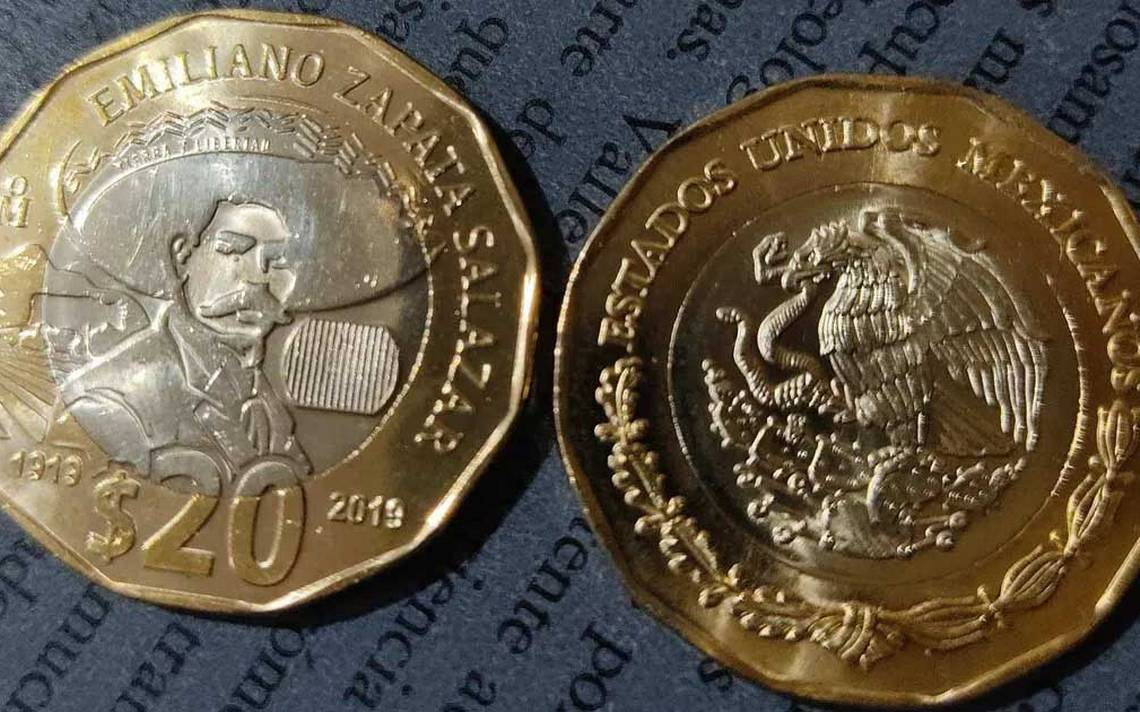
\includegraphics[scale=0.25]{Imagenes/Moneda_Conmemorativa.jpg}
\end{figure}
\end{frame}
\begin{frame}
\frametitle{Arte}
\begin{figure}
    \centering
    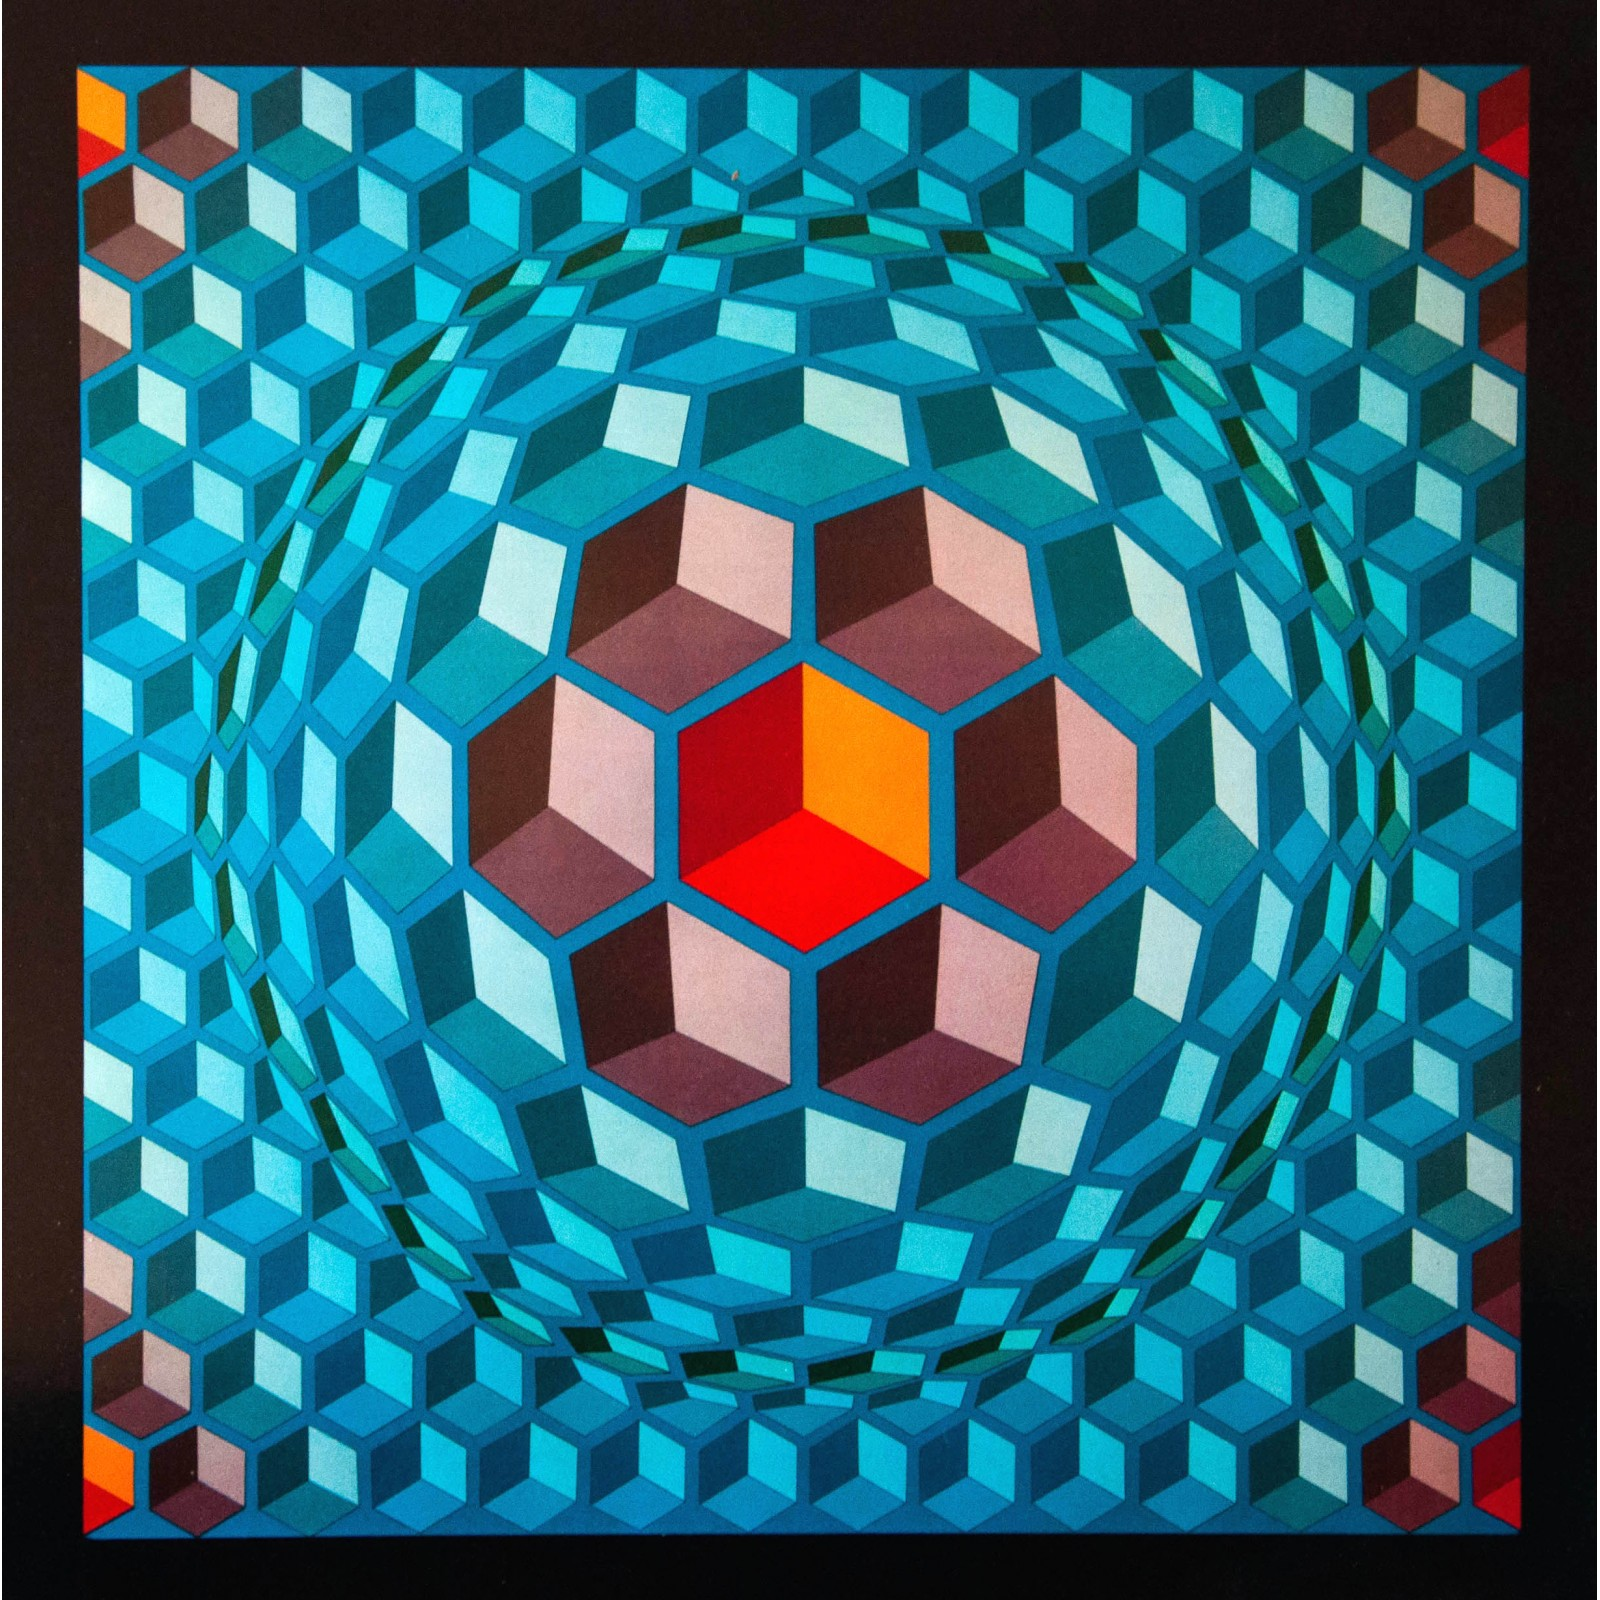
\includegraphics[scale=0.1]{Imagenes/Mosaico_Hexagonal.jpg}
\end{figure}
\end{frame}
\begin{frame}
\frametitle{Arte}
\begin{figure}
    \centering
    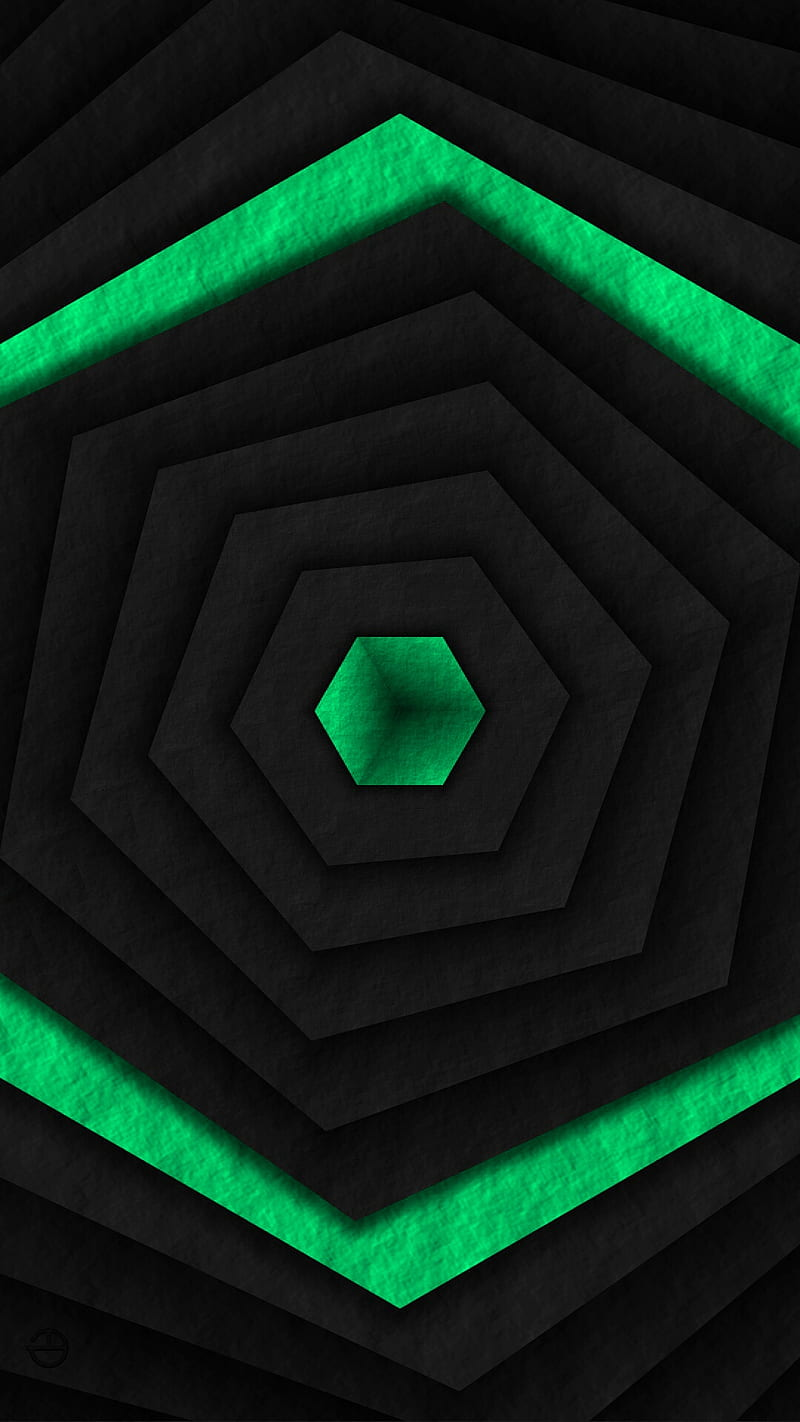
\includegraphics[scale=0.12]{Imagenes/Abstracto_Hexagonal.jpg}
\end{figure}
\end{frame}

\section{Describiendo al polígono}
\frame{\frametitle{Contenido} \tableofcontents[currentsection, hideothersubsections]}
\subsection{Definición}

\begin{frame}
\frametitle{¿Qué es un polígono?}
Llamaremos \textocolor{red}{polígono} a la porción de plano limitada por una curva cerrada: la \textocolor{burgundy}{línea poligonal}.
\end{frame}
\begin{frame}
\frametitle{Etimología}
La palabra \enquote{polígono} proviene del griego \enquote{$\pi o \lambda \upsilon \gamma \omega \nu o \varsigma $} (polugonon), que significa \enquote{muchas esquinas}.
\\
\bigskip
\pause
Está compuesta por \enquote{$\pi o \lambda \upsilon $} (polu-), que significa \enquote{mucho} o \enquote{varios}, \pause y \enquote{$\gamma \omega \nu \iota \alpha $}(gonia), que significa \enquote{esquina} o \enquote{ángulo}.
\end{frame}

\subsection{Características}

\begin{frame}
\frametitle{De los lados}
Los \textocolor{cobalt}{lados} y \textocolor{cadmiumgreen}{vértices} de la línea poligonal, \pause son los lados y vértices del polígono.
\pause
\begin{figure}[t]
    \centering
    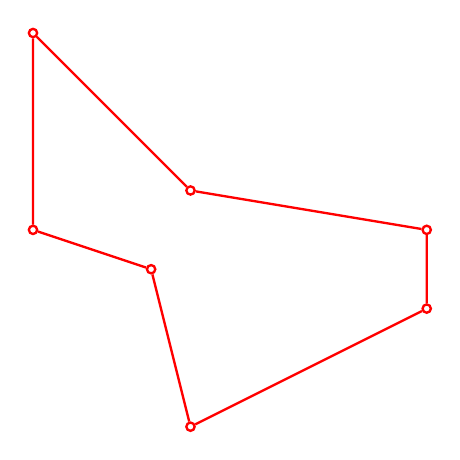
\begin{tikzpicture}[scale=5]
    \tikzstyle{every node}=[draw, fill=white, shape=circle, minimum size=3pt,inner sep=1pt];
    \tikzstyle{every path}=[draw, line width=0.3mm, color=red];
    \node (v1) at (2.2,1) {};
    \node (v2) at (2.8,1.3) {};
    \node (v3) at (2.8,1.5) {};
    \node (v4) at (2.2,1.6) {};
    \node (v5) at (1.8,2) {};
    \node (v6) at (1.8,1.5) {};
    \node (v7) at (2.1,1.4) {};
    \draw (v1)--(v2)--(v3)--(v4)--(v5)--(v6)--(v7)--(v1);
    \end{tikzpicture}
\end{figure}
\end{frame}
\begin{frame}
\frametitle{¿Qué hay de esta figura?}
\begin{figure}
    \centering
    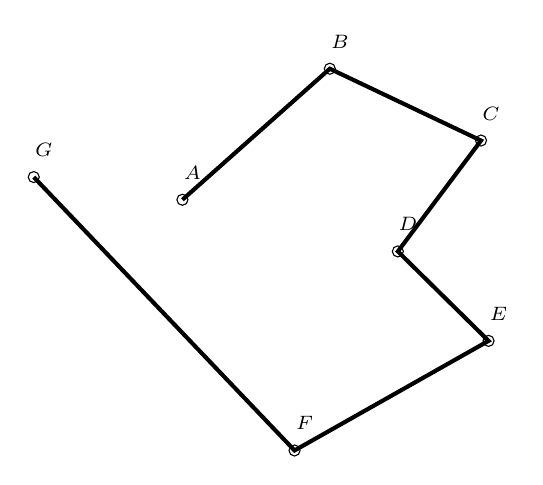
\begin{tikzpicture}[scale=0.8]
        
        \draw [line width=1.5pt] (-6.58,-1.73)-- (-4.24,0.35)-- (-1.84,-0.79)-- (-3.16,-2.55)-- (-1.72,-3.97)-- (-4.8,-5.71)-- (-8.94,-1.37);
        \begin{scriptsize}
            \draw  (-6.58,-1.73) circle (2.5pt);
            \draw (-6.42,-1.3) node {$A$};
            \draw  (-4.24,0.35) circle (2.5pt);
            \draw (-4.08,0.78) node {$B$};
            \draw  (-1.84,-0.79) circle (2.5pt);
            \draw (-1.68,-0.36) node {$C$};
            \draw  (-3.16,-2.55) circle (2.5pt);
            \draw (-3,-2.12) node {$D$};
            \draw  (-1.72,-3.97) circle (2.5pt);
            \draw (-1.56,-3.54) node {$E$};
            \draw  (-4.8,-5.71) circle (2.5pt);
            \draw (-4.64,-5.28) node {$F$};
            \draw  (-8.94,-1.37) circle (2.5pt);
            \draw (-8.78,-0.94) node {$G$};
        \end{scriptsize}
    \end{tikzpicture}
\end{figure}
\end{frame}
\begin{frame}
\frametitle{Ángulos Internos}
Los \textocolor{auburn}{ángulos internos o interiores} de un polígono, \pause son los formados por cada dos lados consecutivos.
\end{frame}
\begin{frame}
\frametitle{Los ángulos internos}
\begin{figure}
    \centering
    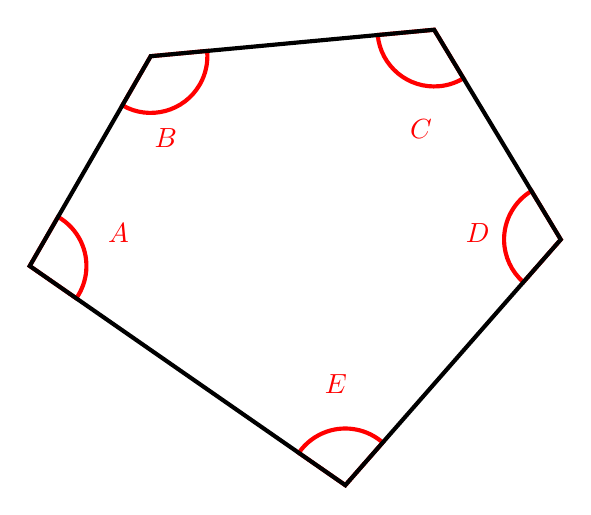
\begin{tikzpicture}[scale=1.2]
                
        \draw [color=red, shift={(-5.86,-0.93)},line width=1.5pt,] (0,0) -- (-119.96674187061168:0.6) arc (-119.96674187061168:5.332158881659562:0.6) -- cycle;
        \draw [color=red, shift={(-2.86,-0.65)},line width=1.5pt] (0,0) -- (-174.66784111834048:0.6) arc (-174.66784111834048:-58.8846676852582:0.6) -- cycle;
        \draw [color=red, shift={(-1.52,-2.87)},line width=1.5pt] (0,0) -- (121.11533231474185:0.6) arc (121.11533231474185:228.75172907052598:0.6) -- cycle;
        \draw [color=red, shift={(-3.8,-5.47)},line width=1.5pt] (0,0) -- (48.751729070525975:0.6) arc (48.751729070525975:145.21573957402293:0.6) -- cycle;
        \draw [color=red, shift={(-7.14,-3.15)},line width=1.5pt] (0,0) -- (-34.78426042597706:0.6) arc (-34.78426042597706:60.03325812938831:0.6) -- cycle;
        
        \draw [line width=1.5pt] (-7.14,-3.15) -- (-5.86,-0.93) -- (-2.86,-0.65) -- (-1.52,-2.87) -- (-3.8,-5.47) -- cycle;

        \draw [line width=0.5pt] (-7.14,-3.15)-- (-5.86,-0.93);
        \draw [line width=0.5pt] (-5.86,-0.93)-- (-2.86,-0.65);
        \draw [line width=0.5pt] (-2.86,-0.65)-- (-1.52,-2.87);
        \draw [line width=0.5pt] (-1.52,-2.87)-- (-3.8,-5.47);
        \draw [line width=0.5pt] (-3.8,-5.47)-- (-7.14,-3.15);
        
        \draw [color=red] (-6.2,-2.8) node {$A$};
        \draw [color=red] (-5.7,-1.8) node {$B$};
        \draw [color=red] (-3,-1.7) node {$C$};
        \draw [color=red] (-2.4,-2.8) node {$D$};
        \draw [color=red] (-3.9,-4.4) node {$E$};
\end{tikzpicture}
\end{figure}
\end{frame}
\begin{frame}
\frametitle{Ángulos Externos}
Los \textocolor{carnelian}{ángulos exteriores o externos} de un polígono, \pause son los ángulos adyacentes a los interiores, obtenidos prolongando los lados en un mismo sentido.
\end{frame}
\begin{frame}
\frametitle{Los ángulos externos}
\begin{figure}
    \centering
    \begin{tikzpicture}[scale=0.7]
        \draw [line width=2pt] (-3,3) -- (2,4) -- (4,1) -- (3,-3) -- (-2,-2) -- cycle;

        \draw [color=ao, shift={(-3,3)},line width=2pt] (0,0) -- (11.309932474020215:0.6) arc (11.309932474020215:100.52078431387436:0.6) -- cycle;
        \draw [color=ao, shift={(-2,-2)},line width=2pt] (0,0) -- (101.30993247402021:0.6) arc (101.30993247402021:162.01266534793857:0.6) -- cycle;
        \draw [color=ao, shift={(2,4)},line width=2pt] (0,0) -- (-56.309932474020215:0.6) arc (-56.309932474020215:11.309932474020227:0.6) -- cycle;
        \draw [color=ao, shift={(4,1)},line width=2pt] (0,0) -- (-104.03624346792648:0.6) arc (-104.03624346792648:-60.4885014429097:0.6) -- cycle;
        \draw [color=ao, shift={(3,-3)},line width=2pt] (0,0) -- (168.6900675259798:0.6) arc (168.6900675259798:252.9622322043744:0.6) -- cycle;

        \draw [line width=2pt] (-3,3)-- (2,4);
        \draw [line width=2pt] (2,4)-- (4,1);
        \draw [line width=2pt] (4,1)-- (3,-3);
        \draw [line width=2pt] (3,-3)-- (-2,-2);
        \draw [line width=2pt] (-2,-2)-- (-3,3);
        \draw [line width=2pt] (2,4)-- (3.4,4.28);
        \draw [line width=2pt] (4,1)-- (4.6,-0.06);
        \draw [line width=2pt] (3,-3)-- (2.62,-4.24);
        \draw [line width=2pt] (-2,-2)-- (-3.54,-1.5);
        \draw [line width=2pt] (-3,3)-- (-3.26,4.4);

        \draw (-2.5,4.01) node [color=ao] {$A$};
        \draw (3, 3.7) node [color=ao] {$B$};
        \draw (4.16, -0.5) node [color=ao] {$C$};
        \draw (1.8, -3.33) node [color=ao] {$D$};
        \draw (-2.76, -1.07) node [color=ao] {$E$};
        
    \end{tikzpicture}
\end{figure}
\end{frame}
\begin{frame}
\frametitle{Los primeros elementos de un polígono}
\begin{figure}
    \centering
    \begin{tikzpicture}
        \draw [line width=2pt] (-2,2) -- (1,2) -- (1.9270509831248424,4.85316954888546) -- (-0.5,6.61652530576288) -- (-2.927050983124842,4.853169548885461) -- cycle;
        
        \draw [line width=2pt] (-2,2)-- (1,2);
        \draw [line width=2pt] (1,2)-- (1.9270509831248424,4.85316954888546);
        \draw [line width=2pt] (1.9270509831248424,4.85316954888546)-- (-0.5,6.61652530576288);
        \draw [line width=2pt] (-0.5,6.61652530576288)-- (-2.927050983124842,4.853169548885461);
        \draw [color=bostonuniversityred] [line width=2pt] (-2.927050983124842,4.853169548885461)-- (-2,2);
        \node at (-4, 3.5) {Lado};
        
        \pause

        \draw [fill=ao] (-2,2) circle (2.5pt);
        \draw [fill=ao] (1,2) circle (2.5pt);
        \draw [fill=ao] (1.9270509831248424,4.85316954888546) circle (2.5pt);
        \draw [fill=ao] (-0.5,6.61652530576288) circle (2.5pt);
        \draw [fill=ao] (-2.927050983124842,4.853169548885461) circle (2.5pt);
        \draw (2.5, 5.2871508154561875) node {Vértice};

        \pause
        \draw [shift={(1,2)},line width=2pt] (0,0) -- (72:0.6048542504621391) arc (72:180:0.6048542504621391) -- cycle;
        \draw [color=red] (0, 2.424174029935399) node {$A$};
        \node at (3, 2.5) [color=red] {Ángulo interno};
        \pause

        \draw [color=ao, shift={(-2,2)},line width=2pt] (0,0) -- (-69.2245017165276:0.6048542504621391) arc (-69.2245017165276:0:0.6048542504621391);
        \draw [line width=2pt] (-2,2)-- (-1.6140255659922953,0.9826047330006348);   
        \draw (-1, 1.5) node {$B$};
        \node at (-3, 1.9) [color=ao, align=center] {Ángulo \\[-0.5em] externo};
\end{tikzpicture}
\end{figure}
\end{frame}
\begin{frame}
\frametitle{La diagonal}
Se llama la \textocolor{cobalt}{diagonal} de un polígono a un segmento que une a dos vértices no consecutivos.
\end{frame}
\begin{frame}
\frametitle{Las diagonales}
\begin{figure}
    \centering
    \begin{tikzpicture}[scale=0.75]
                   
        \draw [line width=2pt] (-3,1) -- (-1.16,2.8) -- (2,1) -- (1.84,-2.44) -- (-2.24,-4.52) -- (-4.88,-2.86) -- cycle;
        
        \draw [line width=2pt] (-3,1)-- (-1.16,2.8);
        \draw [line width=2pt] (-1.16,2.8)-- (2,1);
        \draw [line width=2pt] (2,1)-- (1.84,-2.44);
        \draw [line width=2pt] (1.84,-2.44)-- (-2.24,-4.52);
        \draw [line width=2pt] (-2.24,-4.52)-- (-4.88,-2.86);
        \draw [line width=2pt] (-4.88, -2.86) -- (-3, 1);
        
        \draw [fill=ao] (-3,1) circle (2.5pt);
        \draw [fill=ao] (-3.34,1.57) node {$A$};
        \draw [fill=ao] (-1.16,2.8) circle (2.5pt);
        \draw [fill=ao] (-1,3.23) node {$B$};
        \draw [fill=ao] (2,1) circle (2.5pt);
        \draw [fill=ao] (2.16,1.43) node {$C$};
        \draw [fill=ao] (1.84,-2.44) circle (2.5pt);
        \draw [fill=ao] (2.2,-2.61) node {$D$};
        \draw [fill=ao] (-2.24,-4.52) circle (2.5pt);
        \draw [fill=ao] (-2.24,-4.85) node {$E$};
        \draw [fill=ao] (-4.88,-2.86) circle (2.5pt);
        \draw [fill=ao] (-5.34,-2.69) node {$F$};
        
        \pause
        \draw [color=coquelicot, line width=1.5pt] (-3,1)-- (2,1);
        \pause
        \draw [color=coquelicot, line width=1.5pt] (-3,1)-- (1.84,-2.44);
        \pause
        \draw [color=coquelicot, line width=1.5pt] (-3,1)-- (-2.24,-4.52);

        \pause
        \draw [color=blue, line width=1.5pt, dashed] (-1.16,2.8)-- (-2.24,-4.52);
        \pause
        \draw [color=blue, line width=1.5pt, dashed] (-1.16,2.8)-- (1.84,-2.44);
        \pause
        \draw [color=blue, line width=1.5pt, dashed] (-1.16,2.8) -- (-4.88, -2.86);

    \end{tikzpicture}
\end{figure}
\end{frame}

\subsection{Clasificación de los polígonos}

\begin{frame}
\frametitle{Grupos de polígonos}
Los polígonos se clasifican en tres principales grupos:
\pause
\setbeamercolor{item projected}{bg=black,fg=white}
\setbeamertemplate{enumerate items}{%
\usebeamercolor[bg]{item projected}%
\raisebox{1.5pt}{\colorbox{bg}{\color{fg}\footnotesize\insertenumlabel}}%
}
\begin{enumerate}[<+->]
\item Polígono equilátero.
\item Polígono equángulo.
\item Polígono regular.
\end{enumerate}
\end{frame}
\begin{frame}
\frametitle{Polígono equilátero}
El \textocolor{carmine}{polígono equilátero} es aquel que tiene sus lados iguales y los ángulos internos distintos.
\end{frame}
\begin{frame}
\frametitle{Polígono equilátero}
\begin{figure}
    \centering
    \begin{tikzpicture}
        \draw[line width=2pt, color=cornellred] (1,3) -- (5,3) -- (4,0) -- (0,0) -- cycle;
        \draw [line width=2pt, color=cornellred] (1,3) -- (5,3);
        \draw [line width=2pt, color=cornellred] (5,3) -- (4,0);
        \draw [line width=2pt, color=cornellred] (4,0) -- (0,0);
        \draw [line width=2pt, color=cornellred] (0,0) -- (1,3);
    \end{tikzpicture}
\end{figure}
\pause
\begin{itemize}
\item Lados iguales.
\item Ángulos interiores distintos.
\end{itemize}
\end{frame}
\begin{frame}
\frametitle{Polígono equiángulo}
El \textocolor{darkmagenta}{polígono equiángulo} es aquel donde sus ángulos internos son iguales y los lados son distintos.
\end{frame}
\begin{frame}
\frametitle{Polígono equilátero}
\begin{figure}
    \centering
    \begin{tikzpicture}
        \draw [line width=2pt, color=debianred] (0,0) -- (6,0) -- (6,2) -- (0,2) -- cycle;
        \draw [line width=2pt, color=debianred] (0,0) -- (6,0);
        \draw [line width=2pt, color=debianred] (6,0) -- (6,2);
        \draw [line width=2pt, color=debianred] (6,2) -- (0,2);
        \draw [line width=2pt, color=debianred] (0,2) -- (0,0);
    \end{tikzpicture}
\end{figure}
\pause
\begin{itemize}
\item Ángulos interiores iguales.
\item Lados distintos.
\end{itemize}
\end{frame}
\begin{frame}
\frametitle{Polígono regular}
El \textocolor{firebrick}{polígono regular} es aquel que tiene sus lados y ángulos internos iguales.
\end{frame}
\begin{frame}
\frametitle{Polígono regular}
\begin{figure}
    \centering
    \begin{tikzpicture}
        \draw [line width=2pt, color=halayaube] (0,0) -- (2,0) -- (3,1.7320508075688774) -- (2,3.4641016151377553) -- (0,3.4641016151377557) -- (-1,1.732050807568879) -- cycle;
        \draw [line width=2pt, color=halayaube] (0,0)-- (2,0);
        \draw [line width=2pt, color=halayaube] (2,0)-- (3,1.7320508075688774);
        \draw [line width=2pt, color=halayaube] (3,1.7320508075688774)-- (2,3.4641016151377553);
        \draw [line width=2pt, color=halayaube] (2,3.4641016151377553)-- (0,3.4641016151377557);
        \draw [line width=2pt, color=halayaube] (0,3.4641016151377557)-- (-1,1.732050807568879);
        \draw [line width=2pt, color=halayaube] (-1,1.732050807568879)-- (0,0);
    \end{tikzpicture}
\end{figure}
\pause
\begin{itemize}
\item Ángulos interiores iguales.
\item Lados iguales.
\end{itemize}
\end{frame}

\subsection*{Polígono regular}

\begin{frame}
\frametitle{Centro del polígono regular}
En este tipo de polígonos, notamos sus ejes de simetría con los cuáles podemos obtener su \textocolor{firebrick}{centro \enquote{O}}, \pause que es la intersección de dos de sus ejes de simetría.
\pause
\begin{figure}
    \centering
    \begin{tikzpicture}
        % \draw [line width=2pt, color=halayaube] (0, 0) -- (2, 0) -- (3, 1.7320508075688774) -- (2, 3.4641016151377553) -- (0, 3.4641016151377557) -- (-1, 1.732050807568879) -- cycle;
        \draw [line width=2pt, color=halayaube] (0,0)-- (2,0);
        \draw [line width=2pt, color=halayaube] (2,0)-- (3,1.7320508075688774);
        \draw [line width=2pt, color=halayaube] (3,1.7320508075688774) -- (2,3.4641016151377553);
        \draw [line width=2pt, color=halayaube] (2,3.4641016151377553) -- (0, 3.4641016151377557);
        \draw [line width=2pt, color=halayaube] (0,3.4641016151377557) -- (-1,1.732050807568879);
        \draw [line width=2pt, color=halayaube] (-1,1.732050807568879) -- (0,0);
        \draw [line width=0.75pt] (0, 0) -- (2, 3.4641016151377553);
        \draw [line width=0.75pt] (2, 0) -- (0, 3.4641016151377557);
        \node at (0.5, 1.65) [color=firebrick] {$\mathbf{O}$};
    \end{tikzpicture}
\end{figure}
\end{frame}
\begin{frame}
\frametitle{Ángulo central del polígono regular}
Encontramos también que se forma un \textocolor{red}{ángulo \enquote{C}} con dos segmentos que parten del centro \enquote{O} a los extremos de uno de los lados. \pause
Este ángulo es un \textocolor{red}{ángulo central}.
\pause
\begin{figure}
    \centering
    \begin{tikzpicture}
        \node at (0.5, 1.65) [color=firebrick] {$\mathbf{O}$};

        \draw [line width=2pt, color=halayaube] (0,0) -- (2,0) -- (3,1.7320508075688774) -- (2,3.4641016151377553) -- (0,3.4641016151377557) -- (-1,1.732050807568879) -- cycle;
        \draw [shift={(1.0115578987075386,1.7120319397786867)},line width=1pt,color=red] (0,0) -- (0.4813424884842337:0.6) arc (0.4813424884842337:60.57018431909116:0.6) -- cycle;
        \draw [line width=2pt, color=halayaube] (0,0)-- (2,0);
        \draw [line width=2pt, color=halayaube] (2,0)-- (3,1.7320508075688774);
        \draw [line width=2pt, color=halayaube] (3,1.7320508075688774)-- (2,3.4641016151377553);
        \draw [line width=2pt, color=halayaube] (2,3.4641016151377553)-- (0,3.4641016151377557);
        \draw [line width=2pt, color=halayaube] (0,3.4641016151377557)-- (-1,1.732050807568879);
        \draw [line width=2pt, color=halayaube] (-1,1.732050807568879)-- (0,0);
        \draw [line width=0.8pt] (0,3.4641016151377557)-- (2,0);
        \draw [line width=0.8pt] (2,3.4641016151377553)-- (1.0115578987075386,1.7120319397786867);
        \draw [line width=0.8pt] (1.0115578987075386,1.7120319397786867)-- (0,0);
        \draw [line width=0.8pt] (1.0115578987075386,1.7120319397786867)-- (1.96,1.72);

        \draw[color=red] (1.9, 2.1) node {$\mathbf{C}$};
    \end{tikzpicture}
\end{figure}
\end{frame}
\begin{frame}
\frametitle{Nombrando a los polígonos regulares}
Los polígonos regulares tienen asociado un nombre considerando el número de lados $n$.
\\
\bigskip
\pause
Como veremos, el valor de $n$ será de utilidad para obtener más información sobre los polígonos regulares.
\end{frame}
\begin{frame}
\frametitle{Nombrando los polígonos regulares}
\begin{minipage}{0.4\linewidth}
\begin{table}
\centering
\begin{tabular}{l | l}
$n$ & Nombre \\ \hline
$3$ & Triángulo \\ \hline \pause
$4$ & Cuadrado \\ \hline \pause
$5$ & Pentágono \\ \hline \pause
$6$ & Hexágono \\ \hline
\end{tabular}
\end{table}
\end{minipage}
\pause
\begin{minipage}{0.4\linewidth}
\begin{table}
\centering
\begin{tabular}{l | l}
$n$ & Nombre \\ \hline
$7$ & Heptágono \\ \hline \pause
$8$ & Octágono \\ \hline \pause
$9$ & Eneágono \\ \hline \pause
$10$ & Decágono \\ \hline
\end{tabular}
\end{table}
\end{minipage}
\end{frame}
\begin{frame}
\frametitle{Ángulos del polígono regular}
Revisemos la manera de obtener el valor de los ángulos de un polígono regular:
\pause
\setbeamercolor{item projected}{bg=lava,fg=white}
\setbeamertemplate{enumerate items}{%
\usebeamercolor[bg]{item projected}%
\raisebox{1.5pt}{\colorbox{bg}{\color{fg}\footnotesize\insertenumlabel}}%
}
\begin{enumerate}[<+->]
\item Ángulo central.
\item Ángulo interior.
\item Ángulo exterior.
\end{enumerate}
\end{frame}
\begin{frame}
\frametitle{El ángulo central}
El valor del ángulo central \textocolor{red}{$\angle{C}$} es igual a \ang{360} entre $n$, \pause donde $n$  el número de lados del polígono.
\\[1em]
\pause
\begin{minipage}{0.4\linewidth}
\begin{align*}
\angle{C} = \dfrac{\ang{360}}{n}
\end{align*}
\end{minipage}
\begin{minipage}{0.5\linewidth}
\begin{figure}
    \centering
    \begin{tikzpicture}[scale=0.8]
        % \node at (0.5, 1.65) [color=firebrick] {$\mathbf{O}$};
        \draw [line width=2pt, color=halayaube] (0,0) -- (2,0) -- (3,1.7320508075688774) -- (2,3.4641016151377553) -- (0,3.4641016151377557) -- (-1,1.732050807568879) -- cycle;
        \draw [shift={(1.0115578987075386,1.7120319397786867)},line width=1pt,color=red] (0,0) -- (0.4813424884842337:0.6) arc (0.4813424884842337:60.57018431909116:0.6) -- cycle;
        \draw [line width=2pt, color=halayaube] (0,0)-- (2,0);
        \draw [line width=2pt, color=halayaube] (2,0)-- (3,1.7320508075688774);
        \draw [line width=2pt, color=halayaube] (3,1.7320508075688774)-- (2,3.4641016151377553);
        \draw [line width=2pt, color=halayaube] (2,3.4641016151377553)-- (0,3.4641016151377557);
        \draw [line width=2pt, color=halayaube] (0,3.4641016151377557)-- (-1,1.732050807568879);
        \draw [line width=2pt, color=halayaube] (-1,1.732050807568879)-- (0,0);
        \draw [line width=0.8pt] (0,3.4641016151377557)-- (2,0);
        \draw [line width=0.8pt] (2,3.4641016151377553)-- (1.0115578987075386,1.7120319397786867);
        \draw [line width=0.8pt] (1.0115578987075386,1.7120319397786867)-- (0,0);
        \draw [line width=0.8pt] (1.0115578987075386,1.7120319397786867)-- (1.96,1.72);
        \draw[color=red] (2.1, 2.1) node {$\mathbf{\angle{C}}$};
    \end{tikzpicture}
\end{figure}
\end{minipage}
\end{frame}
\begin{frame}
\frametitle{El ángulo interno}
La medida del ángulo interior \textocolor{ao}{$\angle{I}$} en un polígono regular es igual a \ang{180}  menos la medida del ángulo central \textocolor{red}{$\angle{C}$}.
\pause
\begin{align*}
\angle{I} = \ang{180} - \angle{C}
\end{align*}
\end{frame}
\begin{frame}
\frametitle{El ángulo exterior}
En el del polígono regular, el ángulo exterior \textocolor{halayaube}{E} mide lo mismo que el ángulo central \textocolor{firebrick}{C}.
\pause
\begin{align*}
\angle{E} = \angle{C}
\end{align*}
\end{frame}
\begin{frame}
\frametitle{Ejemplo: el pentágono}
Calculemos los valores de los ángulos del pentágono, \pause sabemos que $n = 5$.
\pause
\begin{figure}
\centering
\begin{tikzpicture}
    \draw[line width=2pt,color=auburn] (-2,-1) -- (1,-1) -- (1.9270509831248424,1.85316954888546) -- (-0.5,3.61652530576288) -- (-2.927050983124842,1.853169548885461) -- cycle;

    \draw [shift={(-0.5,1.30826265288144)},line width=2pt,color=red,fill=red,fill opacity=0.1] (0,0) -- (12.653876111494784:0.6) arc (12.653876111494784:90:0.6) -- cycle;
    \draw [shift={(-2.927050983124842,1.853169548885461)},line width=2pt,color=ao,fill=ao,fill opacity=0.1] (0,0) -- (-72:0.6) arc (-72:36:0.6) -- cycle;
    \draw [shift={(1,-1)},line width=2pt,color=halayaube,fill=halayaube,fill opacity=0.1] (0,0) -- (-0.7957235527392746:0.6) arc (-0.7957235527392746:72:0.6) -- cycle;
    
    \draw [line width=2pt,color=auburn] (-2,-1)-- (1,-1);
    \draw [line width=2pt,color=auburn] (1,-1)-- (1.9270509831248424,1.85316954888546);
    \draw [line width=2pt,color=auburn] (1.9270509831248424,1.85316954888546)-- (-0.5,3.61652530576288);
    \draw [line width=2pt,color=auburn] (-0.5,3.61652530576288)-- (-2.927050983124842,1.853169548885461);
    \draw [line width=2pt,color=auburn] (-2.927050983124842,1.853169548885461)-- (-2,-1);
    
    \draw [line width=1pt] (-0.5,3.61652530576288)-- (-0.5,1.30826265288144);
    \draw [line width=1pt] (-0.5,1.30826265288144)-- (1.9270509831248424,1.85316954888546);
    \draw [line width=1pt] (-0.5,1.30826265288144)-- (1,-1);
    \draw [line width=1pt] (-0.5,1.30826265288144)-- (-2,-1);
    \draw [line width=1pt] (-0.5,1.30826265288144)-- (-2.927050983124842,1.853169548885461);
    \draw [line width=1pt] (1,-1)-- (2.44,-1.02);

    \draw[color=red] (0.22, 2.23) node {$C$};
    \draw[color=ao] (-2.06, 1.2) node {$I$};
    \draw[color=halayaube] (1.92, -0.39) node {$E$};
\end{tikzpicture}
\end{figure}
\end{frame}
\begin{frame}
\frametitle{Ejemplo: el pentágono}
\begin{minipage}{0.4\linewidth}
\begin{figure}
\centering
\begin{tikzpicture}[scale=0.8]
    \draw[line width=2pt,color=auburn] (-2,-1) -- (1,-1) -- (1.9270509831248424,1.85316954888546) -- (-0.5,3.61652530576288) -- (-2.927050983124842,1.853169548885461) -- cycle;

    \draw [shift={(-0.5,1.30826265288144)},line width=2pt,color=red,fill=red,fill opacity=0.1] (0,0) -- (12.653876111494784:0.6) arc (12.653876111494784:90:0.6) -- cycle;
    \draw [shift={(-2.927050983124842,1.853169548885461)},line width=2pt,color=ao,fill=ao,fill opacity=0.1] (0,0) -- (-72:0.6) arc (-72:36:0.6) -- cycle;
    \draw [shift={(1,-1)},line width=2pt,color=halayaube,fill=halayaube,fill opacity=0.1] (0,0) -- (-0.7957235527392746:0.6) arc (-0.7957235527392746:72:0.6) -- cycle;
    
    \draw [line width=2pt,color=auburn] (-2,-1)-- (1,-1);
    \draw [line width=2pt,color=auburn] (1,-1)-- (1.9270509831248424,1.85316954888546);
    \draw [line width=2pt,color=auburn] (1.9270509831248424,1.85316954888546)-- (-0.5,3.61652530576288);
    \draw [line width=2pt,color=auburn] (-0.5,3.61652530576288)-- (-2.927050983124842,1.853169548885461);
    \draw [line width=2pt,color=auburn] (-2.927050983124842,1.853169548885461)-- (-2,-1);
    
    \draw [line width=1pt] (-0.5,3.61652530576288)-- (-0.5,1.30826265288144);
    \draw [line width=1pt] (-0.5,1.30826265288144)-- (1.9270509831248424,1.85316954888546);
    \draw [line width=1pt] (-0.5,1.30826265288144)-- (1,-1);
    \draw [line width=1pt] (-0.5,1.30826265288144)-- (-2,-1);
    \draw [line width=1pt] (-0.5,1.30826265288144)-- (-2.927050983124842,1.853169548885461);
    \draw [line width=1pt] (1,-1)-- (2.44,-1.02);

    \draw[color=red] (0.22, 2.23) node {$C$};
    \draw[color=ao] (-2.06, 1.2) node {$I$};
    \draw[color=halayaube] (1.92, -0.39) node {$E$};
\end{tikzpicture}
\end{figure}
\end{minipage}
\hspace{0.5cm}
\begin{minipage}{0.5\linewidth}
\begin{eqnarray*}
\begin{aligned}
\angle{C} &= \dfrac{\ang{360}}{5} = \pause \ang{72} \\[0.5em] \pause
\angle{I} &= \ang{180} - \angle{C} = \\[0.5em] \pause
&= \ang{180} - \ang{72} = \pause \ang{108} \\[0.5em] \pause
\angle{E} &= \angle{C} = \pause \ang{72}
\end{aligned}
\end{eqnarray*}
\end{minipage}
\end{frame}
\begin{frame}
\frametitle{Actividad para completar}
En su libreta deberán de anotar:
\begin{itemize}
\item Nombre completo.
\item Ejercicio a resolver.
\end{itemize}
La actividad resuelta aporta $1$ punto sobre la evaluación continua de la asignatura. El profesor firmará en la libreta, cada firma cuenta.
\end{frame}
\begin{frame}
\frametitle{Actividad para completar}
\begin{table}
\centering
\begin{tabular}{c | c | c | c | c }
Polígono & $n$ & A. central & A. interno & A. externo \\ \hline
Hexágono & & & & \\ \hline
Octágono & & & & \\ \hline
Decágono & & & & \\ \hline
Dodecágono & & & & \\ \hline
\end{tabular}
\end{table}
\end{frame}

\section{Perímetro y Área}
\frame{\tableofcontents[currentsection, hideothersubsections]}
\subsection{Perímetro de un polígono regular}

\begin{frame}
\frametitle{El perímetro}
El \textocolor{firebrick}{perímetro $P$} de un polígono es la suma de la longitud de cada uno de los lados $L$. \pause Ejemplo: Con el hexágono donde $n = 6$
\begin{eqnarray*}
\begin{aligned}
P &= L + L + L + L + L + L = \\[0.5em] \pause
&= 6 \cdot L
\end{aligned}
\end{eqnarray*}
\end{frame}
\begin{frame}
\frametitle{Perímetro de un hexágono}
\begin{minipage}{0.4\linewidth}
\begin{figure}
\centering
\begin{tikzpicture}[scale=0.8]
    \draw [line width=2pt,color=auburn] (0,0) -- (2,0) -- (3,1.7320508075688774) -- (2,3.4641016151377553) -- (0,3.4641016151377557) -- (-1,1.732050807568879) -- cycle;
    \draw [line width=2pt,color=auburn] (0,0)-- (2,0);
    \draw [line width=2pt,color=auburn] (2,0)-- (3,1.7320508075688774);
    \draw [line width=2pt,color=auburn] (3,1.7320508075688774)-- (2,3.4641016151377553);
    \draw [line width=2pt,color=auburn] (2,3.4641016151377553)-- (0,3.4641016151377557);
    \draw [line width=2pt,color=auburn] (0,3.4641016151377557)-- (-1,1.732050807568879);
    \draw [line width=2pt,color=auburn] (-1,1.732050807568879)-- (0,0);
    \draw (0.5, -0.12) node[anchor=north west] {L=2 m};
    \draw (2.84,1) node[anchor=north west] {L};
    \draw (2.88,3.12) node[anchor=north west] {L};
    \draw (0.7, 4.2) node[anchor=north west] {L};
    \draw (-1, 3.22) node[anchor=north west] {L};
    \draw (-1, 1) node[anchor=north west] {L};
\end{tikzpicture}    
\end{figure}
\end{minipage}
\begin{minipage}{0.5\linewidth}
\begin{eqnarray*}
\begin{aligned}
P &=  L + L + L + L + L + L = \\[0.5em] \pause
&= 6 \cdot L \\[0.5em] \pause
&= 6 \cdot \SI{2}{\meter} \\[0.5em] \pause
&= \SI{12}{\meter}
\end{aligned}
\end{eqnarray*}
\end{minipage}
\end{frame}

\subsection{El área}

\begin{frame}
\frametitle{El área de un polígono}
El \textocolor{byzantine}{área} de un polígono es la medida interna en dos dimensiones de su superficie plana.
\\
\bigskip
\pause
Las unidades de área representan dos dimensiones y son cuadradas: \pause centímetros cuadrados (\unit{\square\centi\meter}), metros cuadrados (\unit{\square\meter}), kilómetros cuadrados (\unit{\square\kilo\meter}), etc. 
\end{frame}
\begin{frame}
\frametitle{Elemento importante}
Para calcular el área de un polígono, debemos de definir un elemento más: \pause la \textocolor{carmine}{apotema}.
\\
\bigskip
\pause
La \textocolor{carmine}{apotema ($\mathbf{a}$)} de un polígono regular es la menor distancia entre el centro y cualquiera de sus lados. 
\end{frame}
\begin{frame}
\frametitle{Elemento importante}
La \textocolor{carmine}{apotema ($\mathbf{a}$)} es un segmento cuyos extremos son el centro de un polígono regular y el punto medio de cualquiera de sus lados.
\pause
\begin{figure}
\centering
\begin{tikzpicture}
    \draw [line width=2pt,color=auburn] (0,0) -- (2,0) -- (3,1.7320508075688774) -- (2,3.4641016151377553) -- (0,3.4641016151377557) -- (-1,1.732050807568879) -- cycle;
    \draw [line width=2pt,color=auburn] (0,0)-- (2,0);
    \draw [line width=2pt,color=auburn] (2,0)-- (3,1.7320508075688774);
    \draw [line width=2pt,color=auburn] (3,1.7320508075688774)-- (2,3.4641016151377553);
    \draw [line width=2pt,color=auburn] (2,3.4641016151377553)-- (0,3.4641016151377557);
    \draw [line width=2pt,color=auburn] (0,3.4641016151377557)-- (-1,1.732050807568879);
    \draw [line width=2pt,color=auburn] (-1,1.732050807568879)-- (0,0);
    \draw [line width=1pt] (1,1.7320508075688779) -- (1,0);
    
    \draw [fill=black] (1,0) circle (1pt);
    \draw [fill=black] (1,1.7320508075688779) circle (1pt);
    \draw[color=black] (0.76,1.11) node {$a$};
\end{tikzpicture}
\end{figure}
\end{frame}
\begin{frame}
\frametitle{Calculando el área de un polígono}
El área o superficie de un polígono es igual al producto del perímetro ($\mathbf{P}$) por la apotema ($\mathbf{a}$) dividido por dos.
\pause
\begin{eqnarray*}
\begin{aligned}
A &= \dfrac{P \cdot a}{2} = \\[0.5em] \pause
&= \dfrac{n \cdot L \cdot a}{2}
\end{aligned}
\end{eqnarray*}
\end{frame}
\begin{frame}
\frametitle{Ejercicio}
Un ingeniero topógrafo está midiendo un terreno en forma de octágono, el lado del polígono mide $L = \SI{60}{\meter}$ y la apotema $a = \SI{34}{\meter}$.
\\
\bigskip
\pause
¿Cuánto valen el perímetro y el área del terreno?
\end{frame}
\begin{frame}
\frametitle{Calculando el área}
\begin{figure}
\centering
\begin{tikzpicture}
\draw [line width=2pt,color=darkmagenta] (0,0) -- (2,0) -- (3.414213562373095,1.414213562373095) -- (3.414213562373095,3.4142135623730945) -- (2,4.82842712474619) -- (0,4.82842712474619) -- (-1.414213562373095,3.4142135623730954) -- (-1.4142135623730954,1.4142135623730956) -- cycle;
\draw [line width=2pt,color=darkmagenta] (0,0)-- (2,0);
\draw [line width=2pt,color=darkmagenta] (2,0)-- (3.414213562373095,1.414213562373095);
\draw [line width=2pt,color=darkmagenta] (3.414213562373095,1.414213562373095)-- (3.414213562373095,3.4142135623730945);
\draw [line width=2pt,color=darkmagenta] (3.414213562373095,3.4142135623730945)-- (2,4.82842712474619);
\draw [line width=2pt,color=darkmagenta] (2,4.82842712474619)-- (0,4.82842712474619);
\draw [line width=2pt,color=darkmagenta] (0,4.82842712474619)-- (-1.414213562373095,3.4142135623730954);
\draw [line width=2pt,color=darkmagenta] (-1.414213562373095,3.4142135623730954)-- (-1.4142135623730954,1.4142135623730956);
\draw [line width=2pt,color=darkmagenta] (-1.4142135623730954,1.4142135623730956) -- (0,0);

\draw [line width=1.5pt] (1,2.414213562373095) -- (1,0);

\begin{small}
\draw (0.36,-0.42) node[anchor=north west] {L = 60 m};
\draw (1, 1.76) node[anchor=north west] {a = 34 m};
\end{small}

\draw [fill=black] (1,0) circle (1pt);
\draw [fill=black] (1,2.414213562373095) circle (1pt);
\end{tikzpicture}
\end{figure}
\end{frame}
\begin{frame}
\frametitle{Obteniendo los valores}
\begin{minipage}{0.4\linewidth}
\begin{figure}
\centering
\begin{tikzpicture}[scale=0.8]
    \draw [line width=2pt,color=darkmagenta] (0,0) -- (2,0) -- (3.414213562373095,1.414213562373095) -- (3.414213562373095,3.4142135623730945) -- (2,4.82842712474619) -- (0,4.82842712474619) -- (-1.414213562373095,3.4142135623730954) -- (-1.4142135623730954,1.4142135623730956) -- cycle;
    \draw [line width=2pt,color=darkmagenta] (0,0)-- (2,0);
    \draw [line width=2pt,color=darkmagenta] (2,0)-- (3.414213562373095,1.414213562373095);
    \draw [line width=2pt,color=darkmagenta] (3.414213562373095,1.414213562373095)-- (3.414213562373095,3.4142135623730945);
    \draw [line width=2pt,color=darkmagenta] (3.414213562373095,3.4142135623730945)-- (2,4.82842712474619);
    \draw [line width=2pt,color=darkmagenta] (2,4.82842712474619)-- (0,4.82842712474619);
    \draw [line width=2pt,color=darkmagenta] (0,4.82842712474619)-- (-1.414213562373095,3.4142135623730954);
    \draw [line width=2pt,color=darkmagenta] (-1.414213562373095,3.4142135623730954)-- (-1.4142135623730954,1.4142135623730956);
    \draw [line width=2pt,color=darkmagenta] (-1.4142135623730954,1.4142135623730956) -- (0,0);

    \draw [line width=1.5pt] (1,2.414213562373095) -- (1,0);

    \begin{small}
    \draw (0.36,-0.42) node[anchor=north west] {L = 60 m};
    \draw (1, 1.76) node[anchor=north west] {a = 34 m};
    \end{small}

    \draw [fill=black] (1,0) circle (1pt);
    \draw [fill=black] (1,2.414213562373095) circle (1pt);
\end{tikzpicture}
\end{figure}
\end{minipage}
\begin{minipage}{0.5\linewidth}
\begin{eqnarray*}
\begin{aligned}
P &= n \cdot L = \\[0.5em] \pause
&= (8) (\SI{60}{\meter}) = \pause \SI{480}{\meter} \\[1em] \pause
A &= \dfrac{P \cdot a}{2} = \\[0.5em] \pause
&= \dfrac{(\SI{480}{\meter})(\SI{34}{\meter})}{2} = \\[0.5em] \pause
&= \dfrac{\SI{16320}{\square\meter}}{2} = \pause \SI{8160}{\square\meter}
\end{aligned}
\end{eqnarray*}
\end{minipage}
\end{frame}
\begin{frame}
\frametitle{Actividad para completar}
En su libreta deberán de anotar:
\begin{itemize}
\item Nombre completo.
\item Ejercicio a resolver.
\end{itemize}
La actividad resuelta aporta $1$ punto sobre la evaluación continua de la asignatura. El profesor firmará en la libreta, cada firma cuenta.
\end{frame}
\begin{frame}
\frametitle{Actividad para resolver}
\setbeamercolor{item projected}{bg=ao,fg=white}
\setbeamertemplate{enumerate items}{%
\usebeamercolor[bg]{item projected}%
\raisebox{1.5pt}{\colorbox{bg}{\color{fg}\footnotesize\insertenumlabel}}%
}
\begin{enumerate}[<+->]
\item ¿Cuál es el polígono regular cuyo ángulo exterior vale \ang{60}?
\item ¿Cuánto vale el ángulo interno de un octágono?
\item Un kiosco tiene forma de hexágono, calcula su área si mide por lado \SI{5}{\meter} y por apotema \SI{4.6}{\meter}.
\end{enumerate}
\end{frame}

\section{Circunferencia y Círculo}
\frame[allowframebreaks]{\tableofcontents[currentsection, hideothersubsections]}
\subsection{La Cincunferencia}

\begin{frame}
\frametitle{La Circunferencia - Definición}
La circunferencia se define como una \textocolor{cobalt}{curva plana, cerrada, cuyos puntos son equidistantes de otro, el centro, situado en el mismo plano}.
\end{frame}
\begin{frame}
\frametitle{La Circunferencia}
\begin{figure}
    \centering
    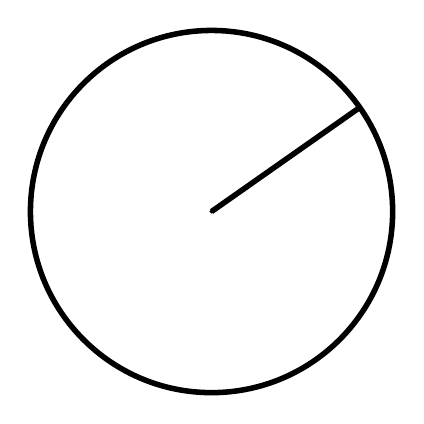
\begin{tikzpicture}
        \draw [line width=2pt] (0,0) circle (2.3cm);
        \draw [line width=2pt] (0,0)-- (1.882349956410611,1.3216499693946844);
        \draw [fill=black] (0,0) circle (0.5pt);
    \end{tikzpicture}    
\end{figure}
\end{frame}

\subsection{Círculo}
\begin{frame}
\frametitle{El círculo - Definición}
Se define como el Círculo al \textocolor{firebrick}{área o superficie plana contenida dentro de una circunferencia}.
\end{frame}
\begin{frame}
\frametitle{El círculo}
\begin{figure}
    \centering
    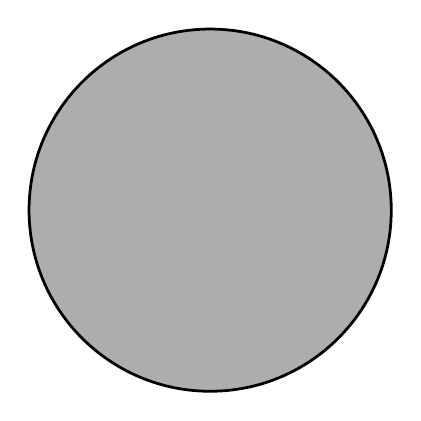
\begin{tikzpicture}
        \draw [line width=1pt,fill=black,fill opacity=0.32] (0,0) circle (2.3cm);
    \end{tikzpicture}
\end{figure}
\end{frame}

\subsection{Elementos del círculo}

\begin{frame}
\frametitle{Elementos del círculo}
\setbeamercolor{item projected}{bg=lava,fg=white}
\setbeamertemplate{enumerate items}{%
\usebeamercolor[bg]{item projected}%
\raisebox{1.5pt}{\colorbox{bg}{\color{fg}\footnotesize\insertenumlabel}}%
}
\begin{enumerate}[<+->]
\item Centro.
\item Radio.
\item Arco.
\item Cuerda.
\item Diámetro.
\item Secante.
\item Tangente.
\end{enumerate}
\end{frame}
\begin{frame}
\frametitle{Elementos del círculo}
El \textocolor{cobalt}{centro} es el punto que está a la misma distancia de todos los puntos pertenecientes a la circunferencia.
\pause
\begin{figure}
    \centering
    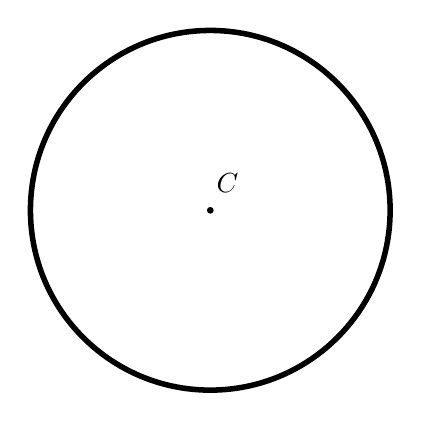
\begin{tikzpicture}
        \draw [line width=2pt] (3,2) circle (2.2840315234251913cm);
        \draw [fill=black] (3,2) circle (1pt);
        \draw[color=black] (3.22,2.35) node {$C$};
    \end{tikzpicture}
\end{figure}
\end{frame}
\begin{frame}
\frametitle{Elementos del círculo}
El \textocolor{red}{radio} es un segmento de recta que une el centro con cualquier punto perteneciente a la circunferencia.
\pause
\begin{figure}
    \centering
    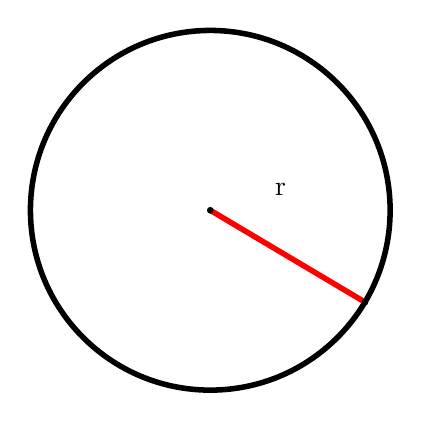
\begin{tikzpicture}
        \draw [line width=2pt] (3,2) circle (2.2840315234251913cm);
        \draw [line width=2pt,color=red] (3,2)-- (4.963935340498931,0.8339133915787598);
        \draw (3.7,2.46) node[anchor=north west] {r};
        \draw [fill=black] (3,2) circle (1pt);
        \draw [fill=black] (4.963935340498931,0.8339133915787598) circle (1pt);
    \end{tikzpicture}
\end{figure}
\end{frame}
\begin{frame}
\frametitle{Elementos del círculo}
El \textocolor{black}{arco} es un segmento de la circunferencia delimitado por dos puntos de la misma.
\begin{figure}
    \centering
    \begin{tikzpicture}
        \draw [line width=1.2pt, dashed] (0,0) circle (2cm);
        \draw [shift={(0,0)},line width=2pt,color=ao]  plot[domain=3.141592653589793:5.395207291363843,variable=\t]({1*2*cos(\t r)+0*2*sin(\t r)},{0*2*cos(\t r)+1*2*sin(\t r)});
        \draw [fill=black] (0,0) circle (1pt);
        \draw [fill=black] (-2,0) circle (1pt);
        \draw [fill=black] (1.2619639312733133,-1.5515949974671883) circle (1pt);
    \end{tikzpicture}
\end{figure}
\end{frame}
\begin{frame}
\frametitle{Elementos del círculo}
La \textocolor{byzantine}{cuerda} es un segmento de recta que une dos puntos cualquiera de una circunferencia.
\pause
\begin{figure}
    \centering
    \begin{tikzpicture}
        \draw [line width=2pt] (3,2) circle (2.2840315234251913cm);
        \draw [line width=2pt,color=ao] (0.8476698966091152,2.764378915222931)-- (4.7757163258948765,3.4365345557801246);
        \draw [fill=black] (0.8476698966091152,2.764378915222931) circle (1pt);
        \draw [fill=black] (4.7757163258948765,3.4365345557801246) circle (1pt);
    \end{tikzpicture}
\end{figure}
\end{frame}
\begin{frame}
\frametitle{Elementos de un círculo}
El \textocolor{carmine}{diámetro} es la mayor cuerda  de una circunferencia. \pause Hay infinitos diámetros y todos pasan por el centro de la circunferencia.
\pause
\begin{figure}
    \centering
    \begin{tikzpicture}[scale=0.8]
        \draw [line width=2pt] (3,2) circle (2.2840315234251913cm);
        \draw [line width=2pt,color=darkgreen] (0.7301778625231852,1.7456233811448398)-- (5.267958315569716,2.27049044130648);
        \draw (2.54,2.94) node[anchor=north west] {d};
        \draw [fill=black] (3,2) circle (1pt);
    \end{tikzpicture}
\end{figure}
\end{frame}
\begin{frame}
\frametitle{Calculando la circunferencia}
Una vez definido el diámetro de un círculo, podemos ocupar este elemento para obtener información del círculo.
\\
\bigskip
\pause
Calculemos el valor de la circunferencia.
\end{frame}
\begin{frame}
\frametitle{Calculando la circunferencia}
Si un círculo tiene un diámetro $\mathbf{d}$
\pause
\begin{figure}
    \centering
    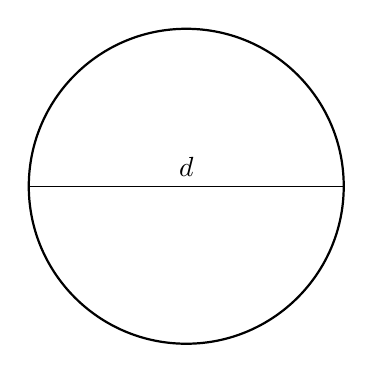
\begin{tikzpicture}
        \draw [thick] (0, 0) circle (2cm);
        \draw (-2, 0) -- (2, 0) node [above, midway] {$d$};
    \end{tikzpicture}
\end{figure}
\end{frame}
\begin{frame}
\frametitle{Relación del diámetro con la circunferencia}
Si cortamos la circunferencia y la extendemos, vamos a medir ahora con el diámetro:
\pause
\begin{figure}
    \centering
    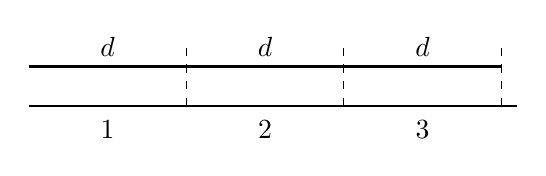
\begin{tikzpicture}
        \draw [thick] (0, 0) -- (6.2, 0);
        \draw [thick] (0, 0.5) -- (2, 0.5) node [above, midway] {$d$};
        \node at (1, -0.3) {$1$};
        \draw [dashed] (2, 0) -- (2, 0.8);
        \pause
        \draw [dashed] (4, 0) -- (4, 0.8);
        \node at (3, -0.3) {$2$};
        \draw [thick] (2, 0.5) -- (4, 0.5) node [above, midway] {$d$};
        \pause
        \node at (5, -0.3) {$3$};
        \draw [thick] (4, 0.5) -- (6, 0.5) node [above, midway] {$d$};
        \draw [dashed] (6, 0) -- (6, 0.8);
        \onslide<1->
    \end{tikzpicture}
\end{figure}

\pause
Vemos que el diámetro \enquote{cabe} tres veces y una pequeña parte en la circunferencia.
\end{frame}
\begin{frame}
\frametitle{Relación del diámetro con la circunferencia}
Encontramos la siguiente relación:
\pause
\begin{align*}
\dfrac{\text{Perímetro} (P)}{\text{diámetro} (d)} = \pi
\end{align*}
\pause
Por lo tanto:
\pause
\begin{align*}
P = \pi \cdot d \hspace{1.5cm} \text{donde } \quad \pi = 3.1416
\end{align*}
El valor de pi ($\pi$) está redondeado.
\end{frame}
\begin{frame}
\frametitle{Relación entre diámetro y radio}
Otra relación importante es la que existe entre el diámetro y el radio de un círculo:
\pause
\begin{align*}
\text{diámetro} = 2 \cdot \text{radio} \hspace{1cm} \Rightarrow \hspace{1cm} d = 2 \cdot r
\end{align*}
\pause
\vspace*{-1cm}
\begin{figure}
    \centering
    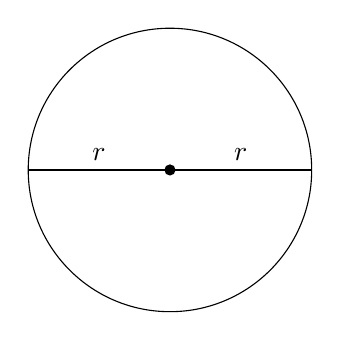
\begin{tikzpicture}[scale=0.9]
        \draw [fill] (0, 0) circle (2pt);
        \draw (0, 0) circle (2cm);
        \draw (0, 0) -- (2, 0) node [above, midway] {$r$};
        \draw (-2, 0) -- (0, 0) node [above, midway] {$r$};
    \end{tikzpicture}
\end{figure}
\end{frame}
\begin{frame}
\frametitle{Expresión equivalente}
Con la relación anterior, podemos ocupar una expresión que nos calcula la circunferencia a partir del radio del círculo:
\pause
\begin{align*}
P = 2 \, \pi \, r
\end{align*}
\end{frame}
\begin{frame}
\frametitle{Expresiones útiles}
El valor de la circunferencia (perímetro) y el área de un círculo, son dos cantidades de mucha utilidad:
\pause
\begin{table}
\centering
\begin{tabular}{l | l | c}
Cantidad & Expresión & Unidades \\ \hline
Perímetro & $P = \pi \cdot d$ & \unit{\meter} \\ \hline
Área & $A = \pi \cdot r^{2}$ & \unit{\square\meter}
\end{tabular}
\end{table}
\end{frame}
\begin{frame}
\frametitle{Elementos de un círculo}
La \textocolor{darkmagenta}{recta secante}, es una recta que corta dos puntos cualesquiera de una circunferencia.
\pause
\begin{figure}
    \centering
    \begin{tikzpicture}[scale=0.8]
        \draw [line width=2pt] (3,2) circle (2.2840315234251913cm);
        \draw [line width=2pt,color=darkmagenta] (0.74,4.04)-- (3.3,-1);
        \draw [fill=black] (3,2) circle (1pt);
    \end{tikzpicture}
\end{figure}
\end{frame}
\begin{frame}
\frametitle{Elementos de un círculo}
La \textocolor{red}{recta tangente}, es una recta que toca a la circunferencia en un solo punto y es perpendicular al radio.
\pause
\begin{figure}
    \centering
    \begin{tikzpicture}[scale=0.75]
        \draw [line width=2pt] (3,2) circle (2.2840315234251913cm);
        \draw [line width=2pt,color=auburn] (3.02,5)-- (6.12,2.38);
        \draw [fill=black] (3,2) circle (1pt);
        \draw [fill=black] (4.469516826105958,3.774924488903997) circle (1pt);
    \end{tikzpicture}
\end{figure}
\end{frame}

\section{Regiones circulares}
\frame{\tableofcontents[currentsection, hideothersubsections]}
\subsection{Sector circular}

\begin{frame}
\frametitle{Actividad a cuenta}
En tu libreta anota el nombre de los elementos del círculo, contará como parte de la evaluación continua de la semana.
\\
\bigskip
\pause
¡Ya tenemos el examen en puerta!
\end{frame}
\begin{frame}
\frametitle{Ejercicio: Nombra los elementos}
\definecolor{ffqqqq}{rgb}{1,0,0}
\begin{figure}
\centering
\begin{tikzpicture}[scale=0.8]
    \draw [line width=2pt] (0,0) circle (2.872211691362599cm);
    \draw [line width=2pt] (-2.3992468998863656,-1.5789915494978637)-- (2.423174388616523,1.5420200654832419);
    \draw [line width=2pt] (0,0)-- (-2.5689842350625667,1.2844921175312838);
    \draw [line width=2pt] (-5.48,1.76)-- (4.8,4.02);
    \draw [line width=2pt] (3.48,2.14)-- (-0.5,-3.96);
    \draw [shift={(0,0)},line width=2pt,color=ffqqqq]  plot[domain=3.922112806897843:4.492958420035007,variable=\t]({1*2.8722116913625984*cos(\t r)+0*2.8722116913625984*sin(\t r)},{0*2.8722116913625984*cos(\t r)+1*2.8722116913625984*sin(\t r)});
    \draw (-0.4,0.82) node[anchor=north west] {A};
    \draw (-1.7,0.62) node[anchor=north west] {B};
    \draw (-0.42,-0.42) node[anchor=north west] {C};
    \draw (-1.82,-2.68) node[anchor=north west] {D};
    \draw (-3.9,3.08) node[anchor=north west] {E};
    \draw (1.6,-1.04) node[anchor=north west] {F};
    \begin{scriptsize}
    \draw [fill=black] (0,0) circle (2.5pt);
    \draw [fill=black] (-2.040843206537579,-2.0210291948236208) circle (1pt);
    \draw [fill=black] (-0.6252054430119738,-2.8033405347956215) circle (1pt);
    \end{scriptsize}
\end{tikzpicture}
\end{figure}
\end{frame}

\begin{frame}
\frametitle{El sector circular}
El \textocolor{auburn}{sector circular} es la región de círculo comprendida entre dos radios.
\pause
\begin{figure}
    \centering
    \begin{tikzpicture}[scale=0.9]
        \draw [shift={(-4,0)},line width=2pt,color=auburn,fill=auburn,fill opacity=0.1] (0,0) -- (0.830315486258011:0.6) arc (0.830315486258011:135:0.6) -- cycle;
        \draw [line width=2pt] (-4,0) circle (2.7602898398537787cm);
        \draw [shift={(-4,0)},line width=2pt,color=auburn,fill=auburn,fill opacity=0.10000000149011612]  (0,0) --  plot[domain=0.014491739065500022:2.356194490192345,variable=\t]({1*2.7602898398537787*cos(\t r)+0*2.7602898398537787*sin(\t r)},{0*2.7602898398537787*cos(\t r)+1*2.7602898398537787*sin(\t r)}) -- cycle ;
        \draw (-5.66,0.94) node[anchor=north west] {r};
        \draw (-3.66,1.82) node[anchor=north west] {$\theta$};
        \draw (-2.88,-0.12) node[anchor=north west] {r};
    \end{tikzpicture}
\end{figure}
\end{frame}
\begin{frame}
\frametitle{Área del sector circular}
El área comprendida en un sector circular, se calcula con la siguiente expresión:

\pause
\begin{minipage}{0.4\linewidth}
\begin{align*}
A = \dfrac{\theta \times \pi}{\ang{360}} \times r^{2}
\end{align*}
\end{minipage}
\begin{minipage}{0.5\linewidth}
    \begin{figure}[scale=0.9]
        \centering
        \begin{tikzpicture}[scale=0.6]
            \draw [shift={(-4,0)},line width=2pt,color=auburn,fill=auburn,fill opacity=0.1] (0,0) -- (0.830315486258011:0.6) arc (0.830315486258011:135:0.6) -- cycle;
            \draw [line width=2pt] (-4,0) circle (2.7602898398537787cm);
            \draw [shift={(-4,0)},line width=2pt,color=auburn,fill=auburn,fill opacity=0.10000000149011612]  (0,0) --  plot[domain=0.014491739065500022:2.356194490192345,variable=\t]({1*2.7602898398537787*cos(\t r)+0*2.7602898398537787*sin(\t r)},{0*2.7602898398537787*cos(\t r)+1*2.7602898398537787*sin(\t r)}) -- cycle ;
            \draw (-5.66,0.94) node[anchor=north west] {r};
            \draw (-3.66,1.82) node[anchor=north west] {$\theta$};
            \draw (-2.88,-0.12) node[anchor=north west] {r};
        \end{tikzpicture}
    \end{figure}
\end{minipage}
\end{frame}
\begin{frame}
\frametitle{Ejemplo con el sector circular}
Calcula el área del siguiente sector circular:
\pause
\begin{figure}
    \centering
    \begin{tikzpicture}[scale=0.9]
        \draw [shift={(-4,0)},line width=2pt,color=darkgreen,fill=darkgreen,fill opacity=0.1] (0,0) -- (0.830315486258011:0.6) arc (0.830315486258011:135:0.6) -- cycle;
        \draw [line width=2pt] (-4,0) circle (2.7602898398537787cm);
        \draw [shift={(-4,0)},line width=2pt,color=darkgreen,fill=darkgreen,fill opacity=0.1]  (0,0) --  plot[domain=0.014491739065500022:2.356194490192345,variable=\t]({1*2.7602898398537787*cos(\t r)+0*2.7602898398537787*sin(\t r)},{0*2.7602898398537787*cos(\t r)+1*2.7602898398537787*sin(\t r)}) -- cycle ;
        \draw (-4, 1.82) node[anchor=north west] {\small{$\theta = \ang{120}$}};
        \draw (-3.5, -0.12) node[anchor=north west] {\small{$r = \SI{3}{\centi\meter}$}};
    \end{tikzpicture}
\end{figure}
\end{frame}
\begin{frame}
\frametitle{Resolviendo el ejercicio}
Presentamos los datos que nos indica el enunciado: \pause $r = \SI{3}{\centi\meter}$ y $\theta = \ang{120}$, \pause por lo que hacemos la sustitución en la ecuación para el área.
\end{frame}
\begin{frame}
\frametitle{Resolviendo el ejercicio}
\begin{eqnarray*}
\begin{aligned}
A &= \dfrac{\theta \times \pi}{\ang{360}} \times r^{2} = \\[0.5em] \pause
&= \left( \dfrac{(\ang{120})(\pi)}{\ang{360}} \right) (\SI{3}{\centi\meter})^{2} = \\[0.5em] \pause
&= \left( \dfrac{\pi}{3} \right) (\SI{9}{\square\centi\meter}) = \pause
 3 \pi \,\, \unit{\square\centi\meter}
\end{aligned}
\end{eqnarray*}
\end{frame}
\begin{frame}
\frametitle{Respuesta al ejercicio}
\begin{figure}
    \centering
    \begin{tikzpicture}[scale=0.9]
        \draw [shift={(-4,0)},line width=2pt,color=darkgreen,fill=darkgreen,fill opacity=0.1] (0,0) -- (0.830315486258011:0.6) arc (0.830315486258011:135:0.6) -- cycle;
        \draw [line width=2pt] (-4,0) circle (2.7602898398537787cm);
        \draw [shift={(-4,0)},line width=2pt,color=darkgreen,fill=darkgreen,fill opacity=0.1]  (0,0) --  plot[domain=0.014491739065500022:2.356194490192345,variable=\t]({1*2.7602898398537787*cos(\t r)+0*2.7602898398537787*sin(\t r)},{0*2.7602898398537787*cos(\t r)+1*2.7602898398537787*sin(\t r)}) -- cycle ;
        \draw (-4, 1.82) node[anchor=north west] {\small{$\theta = \ang{120}$}};
        \draw (-3.5, -0.12) node[anchor=north west] {\small{$r = \SI{3}{\centi\meter}$}};
    \end{tikzpicture}
\end{figure}
\begin{align*}
A = 3 \pi \,\, \unit{\square\centi\meter}
\end{align*}
\end{frame}
\begin{frame}
\frametitle{El segmento circular}
El \textocolor{firebrick}{segmento circular} es la región de círculo comprendida entre una cuerda y su arco.
\pause
\begin{figure}
    \centering
    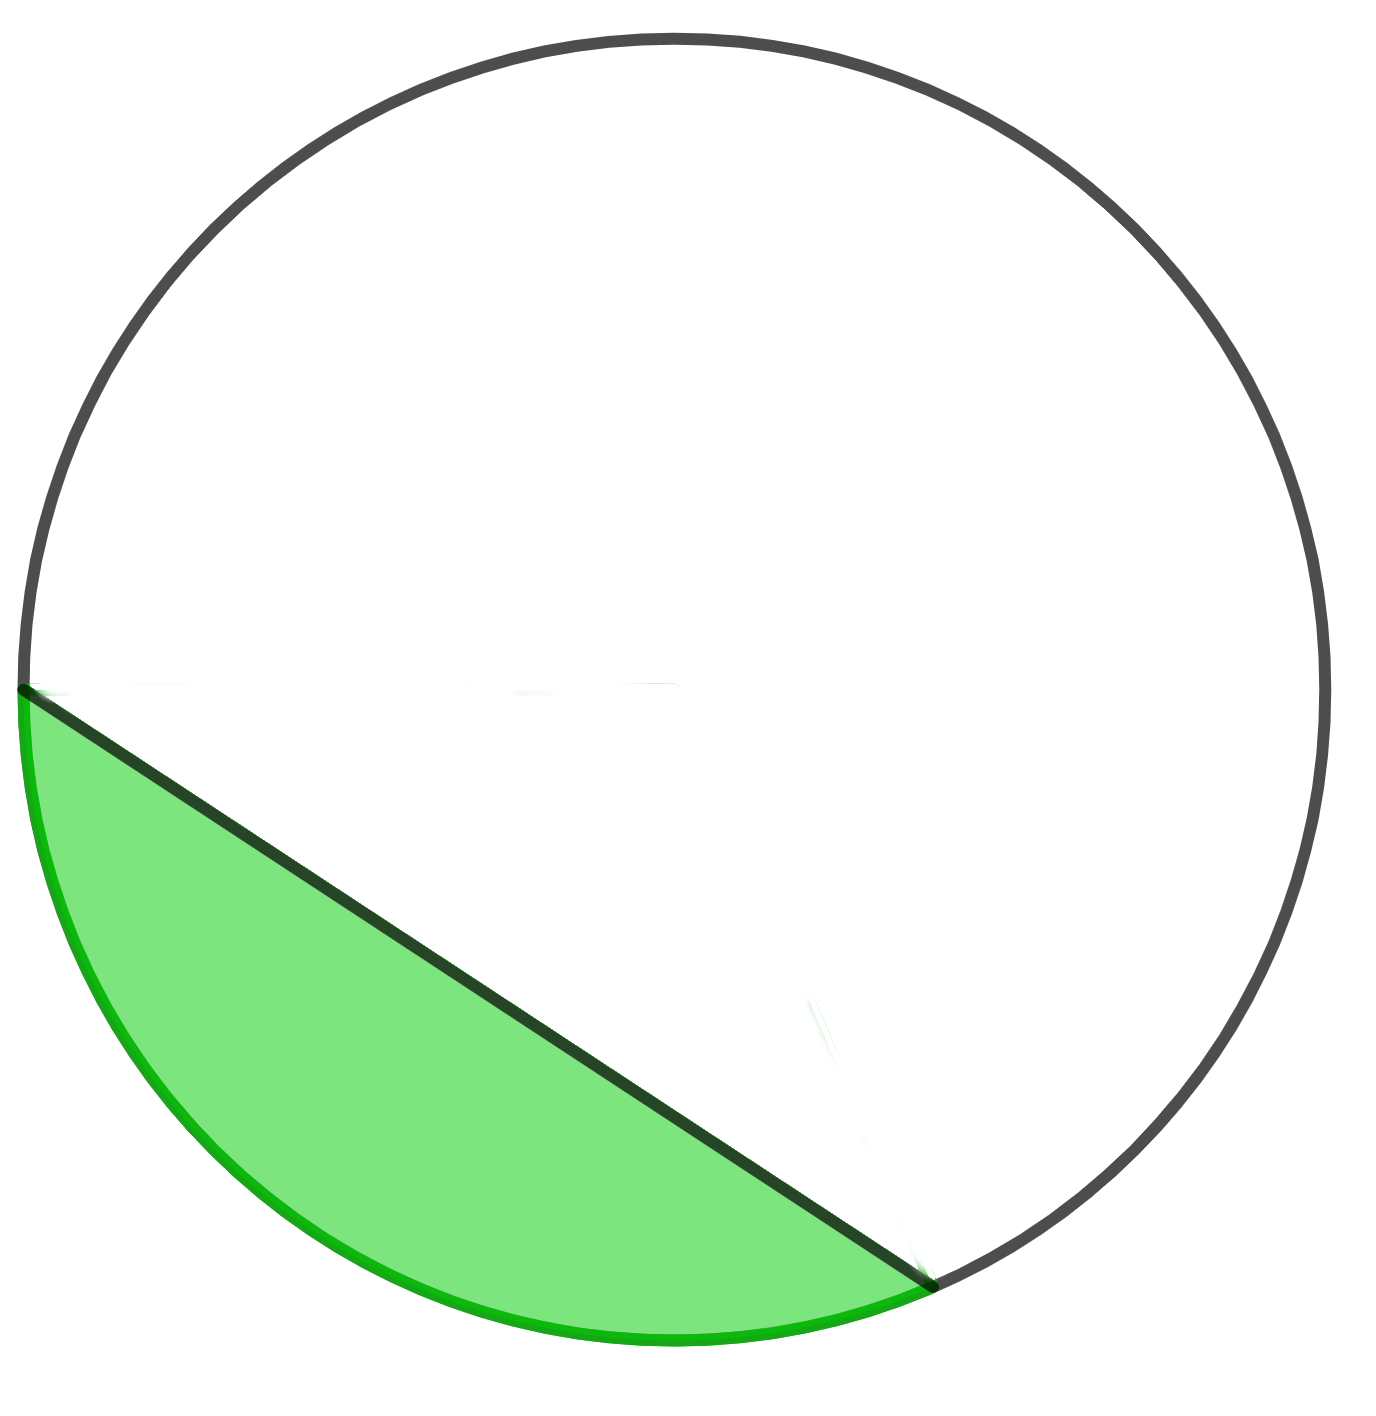
\includegraphics[scale=0.8]{Circulo_Elementos_09.png}
\end{figure}
\end{frame}
\begin{frame}
\frametitle{La corona circular}
La \textocolor{blue}{corona circular} es la porción del plano limitada por dos circunferencias \textocolor{cerise}{concéntricas}.
\end{frame}
\begin{frame}
\frametitle{Circunferencias concéntricas}
Se dice que dos o más circunferencias son \textocolor{cerise}{concéntricas} cuando comparten el mismo centro.
\pause
\begin{figure}
    \centering
    \begin{tikzpicture}
        \draw [thick, color=red] (0, 0) circle (1 cm);
        \draw (0, 0) -- (1, 0) node [above, midway, color=red] {\small{$r_{1}$}};
        \pause
        \draw [thick, color=ao] (0, 0) circle (2 cm);
        \draw (0, 0) -- (0, 2) node [left, midway, color=ao] {\small{$r_{2}$}};
        \pause
        \draw [thick, color=magenta] (0, 0) circle (2.5 cm);
        \draw (0, 0) -- (-2.5, 0) node [below, midway, color=magenta] {\small{$r_{3}$}};
    \end{tikzpicture}
\end{figure}
\end{frame}
\begin{frame}
\frametitle{Circunfencias no concéntricas}
\begin{figure}
    \centering
    \begin{tikzpicture}
        \draw [thick, color=auburn] (0, 0) circle (2 cm);
        \draw [fill] (0, 0) circle (1pt);
        % \draw (0, 0) -- (0, 2) node [left, midway, color=ao] {\small{$r_{2}$}};
        \pause
        \draw [thick, color=red] (2, 0) circle (3 cm);
        \draw [fill] (2, 0) circle (1pt);
        % \draw (0, 0) -- (-2.5, 0) node [below, midway, color=magenta] {\small{$r_{3}$}};
        \pause
        \draw [thick, color=cobalt] (1.5, 1.5) circle (1.5cm);
        \draw [fill] (1.5, 1.5) circle (1pt);
    \end{tikzpicture}
\end{figure}
\end{frame}
\begin{frame}
\frametitle{La corona circular}
\begin{figure}
    \centering
    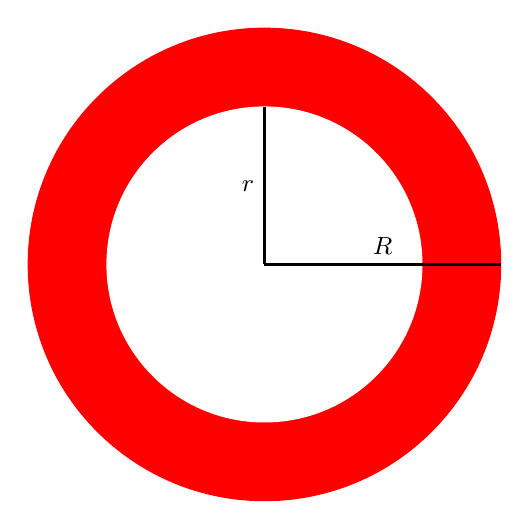
\begin{tikzpicture}
        \draw [draw=black, color=red, fill] (0, 0) circle (3 cm);
        \draw [color=white, fill] (0, 0) circle (2 cm);
        \draw [thick] (0, 0) -- (3, 0) node [above, midway] {\small{$R$}};
        \draw [thick] (0, 0) -- (0, 2) node [left, midway] {\small{$r$}};
    \end{tikzpicture}
\end{figure}
\end{frame}
\begin{frame}
\frametitle{El área de la corona circular}
Para obtener el área de la corona circular debemos de calcular:
\setbeamercolor{item projected}{bg=auburn,fg=white}
\setbeamertemplate{enumerate items}{%
\usebeamercolor[bg]{item projected}%
\raisebox{1.5pt}{\colorbox{bg}{\color{fg}\footnotesize\insertenumlabel}}%
}
\begin{enumerate}[<+->]
\item El área $a_{2}$ del círculo con radio mayor $R$.
\item El área $a_{1}$ del círculo con radio menor $r$.
\item Hacemos la diferencia de las áreas $a_{2} - a_{1}$.
\end{enumerate}
\end{frame}
\begin{frame}
\frametitle{La expresión para el área}
La expresión que nos devuelve el área de una corona circular es:
\pause
\begin{align*}
A = \pi (R^{2} - r^{2})
\end{align*}
\end{frame}
\begin{frame}
\frametitle{Ejemplo de área de corona circular}
Calcula el área de la siguiente corona circular:
\pause
\begin{figure}
    \centering
    \begin{tikzpicture}
        \draw [color=aquamarine, fill] (0, 0) circle (3 cm);
        \draw [color=white, fill] (0, 0) circle (2 cm);
        \draw [thick] (0, 0) -- (3, 0) node [above, midway] {\small{$R = \SI{5}{\centi\meter}$}};
        \draw [thick] (0, 0) -- (0, 2) node [left, midway] {\small{$r = \SI{3}{\centi\meter}$}};
    \end{tikzpicture}
\end{figure}
\end{frame}
\begin{frame}
\frametitle{Usando la expresión}
Se tiene que:
\begin{eqnarray*}
\begin{aligned}
A &= \pi (R^{2} - r^{2}) = \\[0.5em] \pause
&= \pi [ (\SI{5}{\centi\meter})^{2} - (\SI{3}{\centi\meter})^{2}] = \\[0.5em] \pause
&= \pi ( \SI{25}{\square\centi\meter} - \SI{9}{\square\centi\meter}) = \\[0.5em] \pause
&= 14 \, \pi \,\, \unit{\square\centi\meter}
\end{aligned}
\end{eqnarray*}
\end{frame}
\begin{frame}
\frametitle{Ejercicio a cuenta}
El siguiente hexágono de apotema $a = \SI{2}{\centi\meter}$ está inscrito en un círculo con diámetro de \SI{2}{\centi\meter}.
\end{frame}
\begin{frame}
\frametitle{Ejercicio a cuenta}
Calcula el área del círculo que no cubre el hexágono.
\pause
\begin{figure}
\centering
\begin{tikzpicture}
    \fill[line width=2pt,color=auburn,fill=auburn,fill opacity=0.10000000149011612] (-1,0) -- (1,0) -- (2,1.7320508075688774) -- (1,3.4641016151377553) -- (-1,3.4641016151377557) -- (-2,1.732050807568879) -- cycle;
    \draw [line width=2pt,color=auburn] (-1,0)-- (1,0);
    \draw [line width=2pt,color=auburn] (1,0)-- (2,1.7320508075688774);
    \draw [line width=2pt,color=auburn] (2,1.7320508075688774)-- (1,3.4641016151377553);
    \draw [line width=2pt,color=auburn] (1,3.4641016151377553)-- (-1,3.4641016151377557);
    \draw [line width=2pt,color=auburn] (-1,3.4641016151377557)-- (-2,1.732050807568879);
    \draw [line width=2pt,color=auburn] (-2,1.732050807568879)-- (-1,0);
    \draw [line width=2pt] (0,1.7320508075688783) circle (2cm);
\end{tikzpicture}
\end{figure}
\end{frame}
\begin{frame}
\frametitle{Ejercicio a cuenta}
Una corona circular con radios $R$ y $r = \SI{2}{\centi\meter}$, tiene un área de \SI{37.7}{\square\centi\meter}.
\\
\bigskip
\pause
¿Cuánto vale el radio $R$?
\end{frame}

\end{document}